\documentclass[oneside,12pt,fleqn]{memoir}

\usepackage{makeidx}
\usepackage[columns=1]{idxlayout}
%\usepackage[utf8]{inputenc}
\pagestyle{plain}
\binoppenalty2000 \relpenalty2000

%%%%%%%%%%%%%%%%%%%%%%%%%%%%%%%%%%% importa pacchetti
\usepackage{luacode} % load 'luacode' package
\usepackage{usepkg}
%%%%%%%%%%%%%%%%%%%%%%%%%%%%%%%%%%%%% fancyhdr
\usepackage{fancyfoot}
%%%%%%%%%%%%%%%%%% titletoc, titlesec setting
\usepackage{titleT}
%%%%%%%%%%%%%%%%%% setlength
\usepackage{mylength}
\linespread{0.5}

%%%%%%%%%%%% Hyperref package
\usepackage{hyperref}
\hypersetup{colorlinks,
linktoc=all,
linkcolor=black,
    citecolor=black,
    filecolor=black,
    urlcolor=black
}
%%%%%%%%%%%%%%%%%%%%%%%%

%%%%%%%%%%%%%%%%%Geometry package
\usepackage{mygeometry}

%%%%%%%%%%%%%%%%%%%%%%%%%%%%%%%%%%% Funzioni per questo file main
\usepackage{LocalF}
%%%%%%%%%%%%%%%%%%%%%%%%%%%%%%%%%%% Funzioni generali
\usepackage{functions}
%http://tex.stackexchange.com/questions/246/when-should-i-use-input-vs-include
\usepackage{sources}
\usepackage{MathOp}
%%%%%%%%%%%%%%%%%%%%%%%%%%%%%%%%%
%\usepackage{tikz/data}%%import table for tikz pgfplot

\makeindex
\raggedbottom %http://tex.stackexchange.com/questions/102084/annoying-paragraph-spacing-issue-with-memoir 

%%%%%%%%%%%%%%%%%% Import mypackages
%\usepackage{mytitletoc} %% Remeber some problems occurs if you put this after packages
%\usepackage{packages}   %%
%\usepackage{mygeometry} %%
%\usepackage{functions}  %%
%\usepackage{LocalF} %%
%\usepackage{MathOp} %%
%%%%%%%%%%%%%%%%%%% Sources
%\usepackage{sources}
%%%%%%%%%%%%

\author{Pippetta}
\title{Popolazione stellare. Formazione stellare etc}
\date{\today}
%\date{\currenttime}

\makeindex
\raggedbottom %http://tex.stackexchange.com/questions/102084/annoying-paragraph-spacing-issue-with-memoir

%\csname @addtoreset\endcsname{figure}{chapter}
\newcommand{\icgauss}[1]{\directlua{(erfinv(#1))}}
\begin{document}
\icgauss{0.9}
\frontmatter
\maketitle
\addtocontents{toc}{\protect\hypertarget{toc}{}}
\tableofcontents*

\mainmatter

\part{Osservabili stellari. Classificazione}
%\chapter{Massa, distanza, raggio e luminosit\'a. Fotometria, astrometria.}
\PartialToc


%\subsection{Misure di parallasse}

\section{Luminosity function} 

\subsection{Trigonometric parallax}

Stars near the sun: object with total proper motion $\mu>\mu_0$

\subsection{spectroscopic parallax}

To apply this method, one must measure the apparent magnitude of the star and know the spectral type of the star. If the star lies on the main sequence, the spectral type of the star provides a good estimate of the star's absolute magnitude. Knowing the apparent magnitude (m) and absolute magnitude (M) of the star, one can calculate the distance (d, in parsecs) of the star using
\begin{align*}
&M − m = − 5\log{\frac{d}{10}}    
\end{align*}
The true distance to the star may be different than the one calculated due to interstellar extinction.

The spectroscopic absolute magnitude $M$ are derived from the intensity ratio of a number of Fraunhofer lines: the spectroscopic parallax are found using
\begin{equation*}
M=m+5+5\log{\pi_s}-a(\pi_s)
\end{equation*}

\subsection{Comparison of distribution of proper motion components and tangential}



\section{Indicatori di distanza.}

\subsection{Parallasse}

Le coordinate dei corpi celesti osservati dalla superficie terrestre sono topocentriche: la differenza tra diversi punti di osservazione sulla superficie terrestre non \'e trascurabile solo per i corpi del sistema solare e per stelle inferiori a \ang{;;0,00004} essa praticamente non esiste.

Fra le moltitudini di direzioni in cui l'astro \'e visibile dalla superficie quella principale \'e quella con origine nel centro della terra: fornisce la posizione geocentrica dell'astro e determina le sue coordinate geocentriche. L'angolo tra le direzioni secondo cui l'astro $M'$ sarebbe visibile da un qualsiasi punto sulla superficie e dal centro della Terra si chiama parallasse diurna: \'e l'angolo $p'$ sotto il quale dall'astro si vede il raggio della terra per il luogo di osservazione. La parallasse di un astro allo zenit nell'istante di osservazione \'e nulla, se l'astro \'e osservato all'orizzonte la sua parallasse diurna \'e massima ed \'e allora detta parallasse orizzontale $p$.


\subfile{tikz/diurnalparallax.tex}


La relazione fra i lati e gli angoli dei triangoli $TOM'$ e $TOM$ d\'a
\begin{align*}
&\frac{R}{\Delta}=\frac{\sin{p'}}{\sin{z'}},\quad \frac{R}{\Delta}=\sin{p}\\
&\sin{p'}=\sin{p}\sin{z'}
\end{align*}
 La parallasse orizzontale di tutti i corpi del sistema solare \'e molto piccola: Luna $p=\ang{;57;}$, Sole $p=\ang{;;8.79}$, per i pianeti \'e inferiore ad un primo.

I seni delle parallassi possono essere sostituiti con gli angoli stessi: $p'=p\sin{z'}$. 

Poich\'e la forma della Terra \'e quella di uno sferoide si definisce come raggio standard il raggio equatoriale $R_0=6379\si{\kilo\meter}$ e le parallassi orizzontali calcolate per questo raggio si chiamano parallassi orizzontali equatoriali $p_0$.


\subsection{Parallasse.}

Si misura lo spostamento della stella rispetto ad un riferimento di stelle fisse: parallasse diurna $\Delta T=1 \si{\hour}$ (sistema solare), parallasse annua $\Delta T$ di 6 mesi.


\begin{equation*}
    \pi_d=\frac{O_1O_2}{r}=\frac{2r_T\cos{\phi}}{r}
\end{equation*}
cio\'e l'angolo sotteso dalla distanza tra i due punti di osservazione visto dalla stella.

\begin{definition}{Parsec}
Distanza alla quale il semi-asse maggiore dell'orbita terrestre sottende:

\SI{1}{\arcsec}.

\end{definition}

Fatti:
\begin{itemize}
    \item Le stelle pi\'u vicine sono distanti qulache parsec.
    \item Potere risolutivo di un telescopio: $\frac{D}{\lambda}$. Per D=\SI{1}{\meter} e $\lambda=\SI{5000}{\angstrom}$ ho un potere risolutivo di \SI{0.1}{\arcsec}.
    \item Thecniche di best-fit: Numerose osservazioni vs ellissi teorica.
    \item Le osservazioni terrestri sono limitate dal seeing.
\end{itemize}

\subsubsection{Distanze corpi celesti.}

Conoscendo la parallasse equatoriale orizzontale $p_0$ dell'astro si calcola la sua distanza dal centro della terra
\begin{align*}
&\Delta=\frac{R_0}{\sin{p_0}}\\
&\sin{p_0}=p_0''\sin{\ang{;;1}}=\frac{p_0''}{\ang{;;206265}}\\
&\Delta=\frac{\ang{;;206265}R_0}{p_0''}&\intertext{$\uparrow$ le parallassi sono molto piccole: fornisce le distanze dei membri del sistema solare.}
\end{align*}
La distanza del corpo celeste \'e ottenuta nelle stesse unit\'a del raggio  della terra $R_0$.


\subsubsection{Parallasse annua.}

L'angolo sotto cui da una stella si vedrebbe il raggio medio dell'orbita terrestre nella condizione che la direzione verso questa stella sia perpendicolare a questo raggio si chiama parallasse annua $\pi$.

\begin{align*}
&\Delta=\frac{a}{\sin{\pi}}&\intertext{a \'e il raggio medio dell'orbita terrestre. Le parallassi delle stelle sono inferiori a \ang{;;1}:}\\
&\Delta=\frac{\ang{;;206265}a}{\pi''}
\end{align*}

Le parallassi determinate in base allo spostamento parallattico dell'astro sono dette trigonometriche. Le parallasi sono misurate con sufficiente precisione se la loro distanza non supera i 100\si{\parsec} ($\pi=\ang{;;0.01}$): si conoscono le parallassi di circa 6000 stelle vicino al sole.

\subsection{Moto proprio}

Spostamento progressivo rispetto ad un sistema stelle fisse (Blinking): proper motion is the astronomical measure of the observed changes in apparent positions of stars in the sky as seen from the center of mass of the Solar System compared to the imaginary fixed background of the more distant stars.

 This transverse sky motion is separate from the radial velocity, being the velocity moving toward or away from the observer in kilometres per second ($km/s$), as obtained from the Doppler shifts in starlight seen with a spectroscope. Knowledge of the proper motion, distance, and radial velocity allow approximate calculations of a star's true motion in space in respect to the Sun.

Stima distanza:
il moto proprio \'e inversamente proporzionale alla distanza, si deve ipotizzare la conoscenza della velocit\'a relativa rispetto al Sole V. Ipotizzando V costante per stelle vicine e uguale alla velocit\'a del Sole nell'ambiente locale trovo una relazione tra moto proprio sulla sfera celeste u, parallasse e velocit\'a sulla sfera celeste $V_0\sin{\lambda}$ con $\lambda$ angolo tra congiungente stella Sole e direzione del moto del Sole.

\begin{align*}
    &u=\frac{V_0\sin{\lambda}}{4.74}\pi&\intertext{$V_0$ in \si{\kilo\meter\per\second}}\\
    &H=\frac{\pi V_0}{4.74}&\intu{Parallasse secolare}
\end{align*}

Fatti:
\begin{itemize}
    \item Stelle vicine.
    \item Moto proprio progressivo.
    \item Ipotesi V costante applicabile a gruppo di stelle. Parallasse media: 
    \begin{equation*}
        \pi_{media}=\frac{4.74\sum u_i}{V_0\exv{\sin{\lambda}}N}
    \end{equation*}
\end{itemize}

\subsection{Parallasse di gruppo}

Associazione fisica di stelle con stessa velocit\'a relativa rispetto al sole
\begin{equation*}
    V=V_r\hat{r}+V_T\hat{e_T}
\end{equation*}
$V_T$ \'e osservabile mediante effetto Doppler, $V_T$ \'e legata al moto proprio. La parallasse di gruppo \'e 
\begin{equation*}
    \pi_{Gruppo}=\frac{4.74u}{V_R\tan{\lambda}}
\end{equation*}

\subsection{Parallasse statistica}

Ammassi considerati come gas di stelle caratterizzati da distribuzione di velocit\'a isotropa.

\subsubsection{Errore sulla magnitudine assoluta}

\begin{equation*}
    \Delta M_V=2\frac{\Delta\pi}{\pi}
\end{equation*}

\subsection{Unit\'a di misura distanza in astronomia}

\begin{itemize*}
\item Unit\'a astronomica, \si{\astronomicalunit}: Distanza media della Terra dal Sole.
\item \si{\parsec}: distanza corrispondente a una parallase annua di \ang{;;1}.
1\si{\parsec}=\num{30,86e12}\si{\kilo\meter}=\num{206265}\si{\astronomicalunit}=\num{3.26}\si{\lightyear}.
\item anno luce \si{\lightyear}: distanze percorsa in 1 anno dalla luce che viaggia a \num{300000}\si{\kilo\meter\per\second}.
1\si{\lightyear}=\num{9.460e12}\si{\kilo\meter}=\num{63240}\si{\astronomicalunit}=\num{0.3067}\si{\parsec}.
\end{itemize*}

Le distanze nel sistema solare sono espresse in unit\'a astronomiche: mercurio \'e a \num{0.387}\si{\astronomicalunit} dal Sole e Plutone a \num{39,44}\si{\astronomicalunit}.

Le distanze degli astri che si trovano al di fuori del sistema solare sono espresse in \si{\parsec}, \si{\kilo\parsec}, \si{\mega\parsec} ed anche anni luce:
\begin{align*}
&\Delta=\frac{1}{\pi\si{\arcsec}}\si{\parsec}\\
&\Delta=\frac{3.26}{\pi\si{\arcsec}}\si{\lightyear}
\end{align*}

\subsection{Unit\'a astronomica: parallasse del Sole.}

La determinazione diretta della parallasse del sole fornisce risultati grossolani.

Metodo indiretto: parallasse orizzontale di un pianeta che si avvicina alla terra ad una distanza inferiore di quella terra-sole, durante il XX secolo si usava Marte durante le sue opposizioni perieliche (\num{55e6}\si{\kilo\meter}). Supponiamo per semplicit\'a che al momento dell'opposizione perielica il Sole la Terra e Marte siano allineati:

la distanza terra-sole \'e $a_{\odot}=\si{\astronomicalunit}$ e Marte-Sole al perielio \'e $q=a(1-e)$ dove a \'e il semiasse maggiore ed e l'eccentricit\'a dell'orbita marziana, denotiamo con $\parallaxsun$ la parallasse orizontale equatoriale del sole, con $p$ la parallasse orizzontale equatoriale di Marte, con $\Delta$ lasua distanza geocentrica e con $R_0$ il raggio equatoriale della Terra.

\subfile{tikz/sunparallaxM.tex}

\begin{align*}
&R_0=a_0\sin{\parallaxsun}\\
&R_0=\Delta\sin{p}=(q-a_0)\sin{p}\\
&=[a(1-e)-a_0]\sin{p}\\
&a_0\parallaxsun=[a(1-e)-a_0]p&\intu{piccoli angoli, quindi:}\\
&\parallaxsun=[\frac{a}{a_0}(1-e)-1]p&\intu{Il rapporto $\frac{a}{a_0}$ viene calcolato applicando la terza legge di Keplero, mentre la parallasse di Marte p e la sua eccentricit\'a e sono determinate osservativamente.}
\end{align*}

A partire dal 1970:
\begin{equation*}
\parallaxsun=\ang{;;8.794},\quad 1\si{\astronomicalunit}=\num{149.6e6}\si{\kilo\meter}
\end{equation*}

\subsection{Metodi dinamici e fisici}
I metodi dinamici determinano la distanza attraverso la legge di gravitazione universale, i metodi fisici sfruttano la propagazione delle onde radio ($\Delta=\frac{ct}{2}$).


\section{Massa e raggio.}

\subsection{Sole}

La massa la determino usando il moto orbitale della Terra
\begin{align*}
    &\frac{G\msun{}}{d_{T\odot}^2}=\frac{v_T^2}{d_{T\odot}}\\
    &d_{T\odot}=\SI{1}{\astronomicalunit}=\SI{1.496e13}{\cm}\\
    &v_T=\SI{2.978e6}{\cm\per\second}&\intertext{da cui la massa del Sole:}\\
    &\msun{}=\frac{v_T^2d_{T\odot}}{G}=\SI{1.99e33}{\gram}
\end{align*}

e il raggio

\begin{align*}
    &\text{Raggio apparente}=\ang{;15;59.63}\\
    &\rsun{}=\SI{6.96e10}{\cm}
\end{align*}

\subsection{Determinazione della massa}



 \begin{itemize*}
 \item Misurando la gravit\'a alla superficie del corpo considerato.
 
\begin{align*}
g=G\frac{m}{R^2}&\intu{accelerazione di gravit\'a sulla superficie terrestre:}\\
m=\frac{gR^2}{G}
\end{align*}
 
\item Applicando la terza legge di Keplero.

Permette di determinare il rapporto tra la massa del Sole e la massa di un pianeta se questo possiede almeno un satellite e si conosce la distanza satellite-pianeta e il periodo del satellite attorno al pianeta:

\begin{align*}
&\frac{T^2(M+m)}{t_S^2(m+m_S)}=\frac{a^3}{a_S^3}\\
&(\frac{M}{m}+1):(1+\frac{m_S}{m})=\frac{t_S^2a^3}{T^2a_S^3}&\intertext{Il rapporto $\frac{M}{m}$ \'e grande per tutti i pianeti, il rapporto $\frac{m_S}{m}$ \'e piccolo ma in per il sistema Terra-Luna non trascurabile (per i satelliti di Giove si).}
\end{align*}

\item Analizzando le perturbazioni provocate da un astro sui moti di altri corpi celesti.

Le masse dei pianeti senza satelliti sono determinate mediante le perturbazioni create al moto di altri corpi.

\item Red-Shift radiazione.

\end{itemize*}
 

\subsection{Interferometro di Hanbury-brown: Dimensioni angolari.}


\section{Fotometria}
Luminosita' e colore di una stella. la magnitudine (varie definizioni). Sistemi fotometrici, indici di colore e temperatura efficace. 
%http://www.astro.sunysb.edu/fwalter/PHY515/photometry.html


\subsection{Flusso di radiazione osservato}

Sirus \'e 2 miliardi di volte pi\'u brillante della stella pi\'u debole osservata con i telescopi: gran parte della differenza di luminosit\'a apparente \'e dovuta al range di distanze. L'osservazione di ammassi di stelle mostra che $\num{e-6}\lsun{}\leq L\leq \num{e6}\lsun{}$.

\begin{definition}{Stellar photometry}
Tecniche per determinare la luminosit\'a e il colore stellare misurando un range largo dello spettro stellare
\end{definition}


\begin{definition}{Flusso monocromatico $F_{\lambda}$}
$F_{\lambda}$ \'e l'energia emessa dalla stella per unit\'a di tempo, per unit\'a di superficie alla lunghezza d'onda $\lambda$.
\end{definition}

Fatti:
\begin{itemize}
\item Le stelle rapidamente rotanti non hanno forma sferica e la luminosit\'a non \'e uniformemente distribuita sulla superficie
\item La luce riflessa dai pianeti (emissione termica: rilascio energia assorbita) \'e parzialmente anisotropa
\item La simmetria sferica non esiste per emissione non termica: emissione fotoni dovuta al moto di cariche in campo magnetico.
\end{itemize}

\begin{definition}{Luminosit\'a bolometrica.}
\begin{align*}
&L=\int_0^{\infty}L_{\lambda}\,d\lambda=4\pi R^2\int_0^{\infty}F_{\lambda}\\
&L=4\pi R^2\sigma T_e^4,\ \sigma=\num{5.67e-5}(cgs)
\end{align*}
\end{definition}

\begin{align*}
&f_{\lambda}=\frac{\lmono{}}{4\pi r^2}=\lmono{}(\frac{R}{r})^2,\ f=\frac{L}{4\pi r^2}=L(\frac{R}{r})^2&\intu{Flusso di radiazione raccolto da una superficie unitaria: radiazione/superficie * elemento superficie stellare diviso elemento superficie osservatore. Parte della radiazione viene assorbita dal mezzo interstellare e dall'atmosfera}\\
&f_{\lambda}'=A_{\lambda}f_{\lambda}&\intu{effetto assorbimento mezzo interstellare}\\
&f_{\lambda}''=D_{\lambda}(\theta)A_{\lambda}f_{\lambda}&\intu{effetto assorbimento mezzo interstellare e atmosfera}
\end{align*}

\subsubsection{Assorbimento mezzo interstellare}

Discovered in '20: were observed stars whose color temperature were much lower than the temperature indicated by degree of ionization in their spectra (since interstellar reddening follow law similar to temperature reddening). Interstellar reddening was discovered trough comparison of distance of galactic clusters obtained geometrically and photometrically.

Fatti:
\begin{itemize}
\item Is selective with respect to wavelength: increase of observed color index of about \SI{0.31}{\magnitude\per\kilo\parsec}.
\item Doesn't follow Rayleigh's law $I\propto\frac{1}{\lambda^4}$ but varies more nearly as $\frac{1}{\lambda}$.
\end{itemize}

\subsection{Sistemi fotometrici}


\begin{itemize}
    \item UBV: Blue filter is chosen to reduce balmer continuum on blue magnitude. The zero point of blue-yellow color index has been set at A0 
\end{itemize}


\begin{figure}[!ht]
\centering
\includegraphics[width=(0.9\textwidth),height=(\textheight-11mm),keepaspectratio]{obswin}
\caption{Sopra la linea \'e possibile fare astronomia.}
\end{figure}

\begin{definition}{Luce visibile}
Visibile \numrange{3900}{7600}\si{\angstrom}
\end{definition}

\begin{definition}{Curve di sensibilit\'a del rivelatore $S(\lambda)$.}
\begin{itemize}
\item Curva visuale \numrange{5500}{6000}\si{\angstrom}
\item Curva fotografica \numrange{4000}{4500}\si{\angstrom}
\item Curva foto-visuale: riproduce il caso visuale tramite un filtro giallo e una lastra fotografica
\end{itemize}
\end{definition}

\begin{definition}{Larghezza banda (fotometria)}
\begin{itemize}
\item Banda larga: $>100\si{\angstrom}$.
\item Banda media: $\approx100\si{\angstrom}$.
\item Banda stretta: $<100\si{\angstrom}$
\end{itemize}
\end{definition}

\begin{figure}[!ht]
\centering
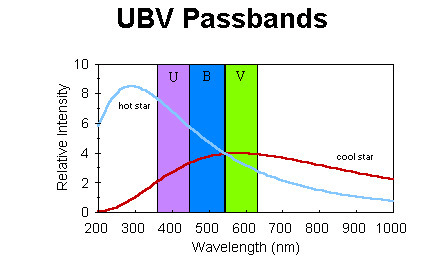
\includegraphics[width=(0.9\textwidth),height=(\textheight-11mm),keepaspectratio]{ubv}
\caption{Filtri passabanda UBV.}
\end{figure}

\clearpage



Sistemi che permettono osservazioni mediante filtri:
\begin{itemize}
\item Johnson-Morgan: (UBV) + 2 filtri VB (fotografici) e un terzo centrato sui \SI{3600}{\angstrom} in corrispondenza del salto di Balmer (FWHM:\SI{900}{\angstrom}, \SI{1000}{\angstrom}, \SI{700}{\angstrom}).
\item Ginevra: (UBV) + filtri nel visibile (a banda stretta)
\item Stromgren: 3 filtri UBV a banda stretta filtro Y intorno ai \SI{4700}{\angstrom} e un filtro centrato su linea idrogeno $H\beta$ ($2\to4$).
\item WUBV: band ($\lambda,\ \Delta\lambda$\si{\angstrom}) W($3270,\ 150$), U($3670,\ 260$), B($4295,\ 420$), V($5450,\ 850$)
\end{itemize}

Risposta di un Fotometro (visuale):
\begin{align*}
&f(\lambda)=S_VD_{\lambda}(\theta)A_{\lambda}f_{\lambda}\\
&I_V=\int_0^{\infty}f(\lambda)\,d\lambda\\
&=\int_0^{\infty}S_VD_{\lambda}(\theta)A_{\lambda}\lmono{}\frac{\,d\lambda}{4\pi r^2}
\end{align*}

Fatti:

\begin{itemize}
\item Wide band photometry: $B-V$. Limited by interstellar absorption.
\item Narrow band photometry: Strenght $H\gamma,\ H\delta$ to luminosity.
\item Ultraviolet method: Barbier-Chalonge, Balmer discontinuity at \mblock{\lambda=\SI{3647}{\angstrom}}.
\item Photographic method: ratio of absorption-line pairs.
\end{itemize}


\subsection{Magnitudine relativa}

In 1856, Norman Robert Pogson formalized the system by defining a first magnitude star as a star that is $100$ times as bright as a sixth-magnitude star, thereby establishing the logarithmic scale still in use today. This implies that a star of magnitude $m$ is $2.512$ times as bright as a star of magnitude $m+1$.

\subsubsection{Formula gi Pogson}

\begin{definition}{Magnitudine relativa}
\begin{equation*}
m_V=-2.5\log{I_V}+\const{}
\end{equation*}

Magnitudine di riferimento:
\begin{equation*}
-2.5\log{I_V*}+\const{}=0
\end{equation*}

\end{definition}

Vega ($\alpha$-Lyr)  ha magnitudine relative circa zero.

\subsection{Magnitudine assoluta}

Absolute magnitude is the measure of intrinsic brightness of a celestial object. It is the hypothetical apparent magnitude of an object at a standard distance of exactly \SI{10}{\parsec} (\SI{32.6}{\lightyear}) from the observer, assuming no astronomical extinction of starlight. This places the objects on a common basis and allows the true energy output of astronomical objects to be compared without the distortion introduced by distance. As with all astronomical magnitudes, the absolute magnitude can be specified for different wavelength intervals; for stars the most commonly quoted absolute magnitude is the absolute visual magnitude, which uses only the visual (V) band of the spectrum (UBV system). Also commonly used is the absolute bolometric magnitude, which is the total luminosity expressed in magnitude units that takes into account energy radiated at all wavelengths, whether visible or not.

\begin{definition}{Magnitudine assoluta}
\begin{equation*}
M_V=m_V+5\log{\frac{\SI{10}{\parsec}}{r}}-A
\end{equation*}
r \'e la distanza della stella (in pc), A rappresenta l'assorbimento interstellare (media di $\log{A_{\lambda}}$) dipende dalla distanza ed \'e massimo sul piano galattico ($\exv{A}\approx\frac{r}{2000\si{\parsec}}$).
\end{definition}

\begin{definition}{Magnitudine bolometrica.}
\'E la magnitudine che otterremmo raccogliendo tutta la luce che giunge all'orbita terrestre (\mblock{A_{\lambda}S_{\lambda}(\theta)=1}). Introduco la correzione bolometrica $BC$:
\begin{equation*}
m_{Bol}=m_V+BC
\end{equation*}
Scelgo che $BC\approx0$ per stelle che emettono nel visibile.
\end{definition}

Fatti:
\begin{itemize}
\item Allen (2000): $BC=0$ per supergiganti di classe di luminosit\'a 1 e tipo $F2$.
\end{itemize}

\begin{definition}{Magnitudine bolometrica assoluta.}
Magnitudine bolometrica assoluta:
\begin{align*}
&M_{Bol}=-2.5\log{\frac{L}{\lsun{}}}+4.74&\intertext{$4.74$ sarebbe la magnitudine bolometrica assoluta del sole se fosse a \SI{10}{\parsec}}\\
&(\lsun{}=\SI{3.845e33}{\erg\per\second})
\end{align*}
\end{definition}

\clearpage

\subsection{Indici di colore.}

\begin{definition}{Indicatori bande sistemi fotometrici}
Zona dello spettro: Lettera del filtro, Punto medio della radiazione effettiva  $\lambda_{eff}$
per il filtro standard, $FWHM$, Variante/i,	Descrizione.
\begin{itemize}

\item   Ultravioletto:
 U , $365 nm$ ,	$66 nm$ ,	$u, u', u*$,	"U" sta per "ultravioletto".
 
\item Visibile:

B, $445 nm$ , $94 nm$, $b$,	"B" sta per "blu".

V,	$551 nm$ , $88 nm$, $v, v'$, "V" sta per "visibile".

G, , , $g, g'$, "G" sta per "green" (verde).

R, $658 nm$, $138 nm$, $r, r', R', Rc, Re, Rj$, "R" sta per "rosso".

\item Infrarosso vicino:

I, $806 nm$, $149 nm$, $i, i', Ic, Ie, Ij$, "I" sta per "infrarosso".

Z ,,, z, z',.

Y $1020 nm$, $120 nm$, $y$,.

J, $1220 nm$, $213 nm$, $J', Js$,.

H, $1630 nm$, $307 nm$,,,.

K, $2190 nm$, $390 nm$, $K$, Continuum, K', Ks, Klong, K8, nbK.

L, $3450 nm$, $472 nm$, $L', nbL'$,.

\item Infrarosso medio:

M, $4750 nm$, $460 nm$, $M', nbM$,.	
N , , , $N1, N2, N3$,.

Q, , ,$ Q'$,.
 	
\end{itemize}     

\end{definition}

\begin{align*}
&U-B=m_U-m_B\\
&B-V=m_B-m_V&\intertext{Una stella blu ha $B-V$ pi\'u basso di una stella rossa.}
\end{align*}

Fissiamo le costanti per avere per stelle $A0$
\begin{equation*}
m_V\approx m_B\approx m_U
\end{equation*}
La distanza provoca uno spostamento verso il rosso: $E(B-V)\approx0.3 A$, $E(U-B)\approx0.1A$.

\subsection{SAAO Standards for Optical Photometry}

\begin{itemize}
    \item Harvard E-Region. 48 equal areas into which Pickering divided the sky
    \item $UBVR_cI_c$. optical UBV + R e I. The colour $(V-I)_C$ is a good temperature indicator that is less sensitive to gravity effects than $(B-V)$, $(U-B)$ is strongly affected by H Balmer absorption: together these 3 colors are usefull to determine color excess of stars (scattering/absorption of star light by interstellar dust).
    \item Str\"omgren $uvby$. Intermediate-band photometric system, narrower band. Metallicity index \mblock{m_1=(v-b)-(b-y)}. The index \mblock{c_1=(u-v)-(v-b)} is a mesure of Balmer discontinuity and thus a T index for OB stars and a surface gravity index for AF stars.
    \item $H\beta$. Intermediate pass-band (\mblock{FWHM\approx\SI{150}{\angstrom}}) and a narrow pass-band (\mblock{FWHM\approx\SI{30}{\angstrom}}) both centered on the Balmer $H\beta$ line of Hydrogen. A magnitude difference between the two filter measure the strength of $H\beta$: good surface gravity/luminosity index for OB stars and good T index for AF stars
    \item DDO. Intermediate pass-band filters (and narrow filter), $FWHM\approx\SI{80}{\angstrom}$. The system was intended for measure integrated light from galaxy nuclei to construct stellar population model for galaxies. The six pass-band are centered between \SIrange{3500}{4800}{\angstrom} and colours of the form $C(35-38)$, $C(38-41)$, \ldots are derived giving parameter related to Balmer discontinuity, line blanketing near \SI{4100}{\angstrom}, strength of CN absorption and G-band break. Usefull for F-K type stars.
\end{itemize}



\section{Stelle doppie.}

\begin{todo}{Stelle doppie}
Le stelle doppie: metodi di osservazione, problematiche generali; effetti di selezione. le stelle doppie per la stima delle masse e dei raggi delle stelle. relazioni massa-raggio e massa-luminosit\'a. 
\end{todo}


Circa la met\'a delle stelle osservate fanno parte di un sistem binario e in sistemi multipli si hanno spesso sottosistemi doppi poco influenzati dalle altre masse.

Dal moto orbitale posso ricavare in situazioni favorevoli
\begin{itemize}
    \item Somma delle masse
    \item Rapporto delle masse
    \item (Luminosit\'a delle componenti)
    \item Periodo orbitale
\end{itemize}


\subsection{Binarie visuali.}

Separazione angolare minore osservabile:

\SI{1}{\arcsec} dalla Terra, limitata dalle dimensioni del telescopio dallo spazio (circa \SI{e-2}{\arcsec}).

I sistemi pi\'u facilmente osservabili sono quelli a periodo lungo (grande separazione) e non troppo distanti:

un sistema a \SI{100}{\parsec} ha separazione \SI{1}{\arcsec} se \'e largo \SI{100}{\astronomicalunit} (per masse solari il periodo \'e di centinaia di anni).

Quindi le regole di selezione porteranno ad osservare con maggior frequenza sistemi vicini e di periodo lungo ma osservabile con stessa luminosit\'a delle componenti (sistemi gemelli).

Masse e raggi.

Terza legge di Keplero:
\begin{align*}
    &M_1+M_2=\frac{4\pi^2a^3}{GP^2}\\
    &M_1+M_2=\frac{1}{P^2}(\frac{a}{\Pi})^3&\intu{P in anni solari, a in arcsec, M's in $\msun{}$}
\end{align*}

quindi nota la parallasse $\Pi$, osservati $P$ e $a$ si ricava la somma delle masse.

Per ricavare le masse analizzo il moto delle due componenti rispetto al CM:

\subfile{tikz/binaryV}

\begin{equation*}
    \frac{M_1}{M_2}=\frac{a_2}{a_1}
\end{equation*}

\subsection{Binarie spettroscopiche.}

Misura la variazione periodi della velocit\'a radiale misurata tramite effetto Doppler.

Classi di oggetti privilegiati:
\begin{itemize}
    \item Oggetti non troppo deboli: spettro a media dispersione.
    \item Periodi non troppo lunghi: un periodo di $T\approx\SI{100}{\year}$ per masse solari comporta una $V_R\approx\SI{1}{\kilo\meter\per\second}$ (difficile da osservare), un periodo $T\approx\SI{1}{\year}$ comporta una $V_R\approx\SI{10}{\kilo\meter\per\second}$.
    \item A seconda del rapporto fra le luminosita sono osservabili una sola o entrambe le componenti.
\end{itemize}

Masse e raggi.
Sistema non risolto spazialmente, tengo conto dell'inclinazione del piano dell'orbita rispetto al piano notmale alla linea di vista moltiplicando ambo i membri della terza legge di Keplero per $\sin{i}$:

\begin{equation*}
    (M_1+M_2)\sin^3{i}=\frac{4\pi a^3\sin^3{i}}{GP^2}
\end{equation*}

Se sono note le velocit\'a radiali di ambo le componenti da \mblock{\frac{M_1}{M_2}=\frac{a_2\sin{i}}{a_1\sin{i}}=\frac{v_{2R}}{v_{1R}}} ottengo \mblock{M_1\sin^3{i}$ e $M_2\sin^3{i}}.

Se \'e nota solo una componente posso misurare
\begin{align*}
    &\frac{4\pi^2}{GP^2}a_1^3\sin^3{i}=(M_1+M_2)\sin^3{i}\frac{M_2^3}{(M_1+M_2)^3}&\intertext{quindi}\\
    &a=a_1+a_2=a_1(1+\frac{a_2}{a_1})=a_1(1+\frac{M_1}{M_2})\\
    &=a_1\frac{(M_2+M_1)}{M_2}
\end{align*}

Definisco la funzione di massa

\begin{equation*}
    f(M_1,M_2)=\frac{v_1^3P}{2\pi G}=\frac{(M_2\sin^3{i})^3}{(M_1+M_2)^2}
\end{equation*}

Fatti:
\begin{itemize}
    \item Se il sistema \'e anche fotometrico posso ricavare $\sin{i}$.
    \item Per $i=\frac{\pi}{2}$ ottengo un limite inferiore per le masse.
\end{itemize}

\subsection{Binarie a eclisse (fotometriche).}

Tecniche fotometriche: eclisse parziale/totale fra le componenti.

Osservabilit\'a dipende da inclinazione del piano dell'orbita rispetto alla linea di vista: l'angolo massimo dipende dalle dimensioni degli astri e dalla loro separazione.

Fatti:
\begin{itemize}
    \item Un periodo di un anno fra 2 stelle simili al Sole permette eclissi se l'angolo fra la linea di vista e il piano dell'orbita \'e minore di \ang{1;;}
    \item Separazione di pochi raggi stellari: per stelle non giganti periodo di giorni.
\end{itemize}

Masse e raggi.

\begin{figure}[!ht]
\centering
\includegraphics[width=\textwidth,height=0.9\textheight,keepaspectratio]{binaryE}
\caption{Binarie a eclisse.}\label{fig:binaryE}
\end{figure}

Analisi curva di luce (vedi \ref{fig:binaryE}):

\begin{align*}
    &M_1+M_2=\frac{4\pi^2a^2}{P^2G}&\intu{Terza legge di Keplero,}\\
    &\frac{t_4-t_1}{P}=\frac{2(R_L+R_S)}{2\pi a}\\
    &\frac{t_3-t_2}{P}=\frac{2(R_L-R_S)}{2\pi a}&\intertext{quindi ricavo $\frac{R_L}{a}$, $\frac{R_S}{a}$.}
\end{align*}

Ricavo le relazioni semi-empiriche per le stelle della MS \index{Relazioni semiempiriche MS.}:

\begin{align*}
    &R\propto M\expy{\frac{1}{2}}\\
    &L\propto \left\{\begin{array}{c}
         M^4,\ M<0.8\msun{}  \\
         M^3,\ M>0.8\msun{}  \\
    \end{array}\right.
\end{align*}

\clearpage


\chapter{Spettri stellari: Spettroscopia.}
\PartialToc

\section{Formazione spettri stellari: righe di assorbimento.}
Classificazione degli spettri stellari. Classi di luminosit\'a. 
Elementi di teoria delle righe spettrali. larghezza naturale di una riga. Introduzione ai fenomeni di allargamento. 
Allargamento delle righe spettrali: vari effetti. Spettri ad alta, media e bassa dispersione.

\subsection{Emission Line (Nebulae)}

Strong emission line owing to allowed/forbidden transitions of heavy elements (N, O, Ne, S, Cl, Ar, P, Fe, Ca, Mn, Cr, V, Co, Ni) in varous ionization stages: allowed transition are accounted for by electric dipole radiation, whereas forbidden transitions are due to magnetic dipole / electric quadrupole radiation. Forbidden emeission lines result from collisional excitation of metastable levels were first identified in gaseus nebula by Bowen (1928).


\subsubsection{Idrogeno}

\begin{definition}{Salto di Balmer}
Balmer jump or Balmer discontinuity is the difference of intensity of the stellar continuum spectrum on both sides of the limit of the Balmer series of hydrogen at \SI{364.6}{\nano\meter}. It is caused by electrons being completely ionized directly from the second energy level of a hydrogen atom (bound-free absorption), which creates a continuum absorption at wavelengths shorter than \SI{364.6}{\nano\meter}.

In some cases the Balmer discontinuity can show continuum emission, usually when the Balmer lines themselves are strongly in emission. Other hydrogen spectral series also show bound-free absorption and hence a continuum discontinuity, but the Balmer jump in the near UV has been the most observed.

The strength of the continuum absorption, and hence the size of the Balmer jump, depends on temperature and density in the region responsible for the absorption. At cooler stellar temperatures, the density most strongly affects the strength of the discontinuity and this can be used to classify stars on the basis of their surface gravity and hence luminosity. This effect is strongest in A class stars, but in hotter stars temperature has a much larger effect on the Balmer jump than surface gravity.
\end{definition}

\begin{definition}{Serie di Balmer}
\begin{figure}[!ht]
\centering
\includegraphics[width=(0.9\textwidth),height=(\textheight-11mm),keepaspectratio]{Bserie}
\caption{Serie di Balmer.}
\end{figure}
\end{definition}

\subsection{Atmosfera stellare}

Lo spettro di una stella \'e caratterizzato da una distribuzione simile a quella di un corpo nero per cui si pu\'o definire una lunghezza d'onda di massima emissione e da righe di assorbimento che danno informazioni sulla struttura chimico-fisica dell'atmosfera: lo spettro risulta dai fotoni provenienti dagli strati esterni dell'atmosfera fino ad una certa profondit\'a ottica e dal loro assorbimento negli strati attraversati.

\begin{usefull}{Radiative transfer equation}
\begin{align*}
&\mu\TDy{I_{\nu}}{\tau_{^nu}}=I_{\nu}-S_{\nu}&\intertext{$S_{\nu}$ is the source function ratio between emission and ambsorption coefficients, in thermodynamic equilibrium $B_{\nu}(T)$ is the source function:}\\
&j_{\nu}=\kappa_{\nu a}\frac{cu_{\nu}}{4\pi}=\kappa_{\nu a}B_{\nu}(T)\\
&d\tau_{^nu}=-\kappa_{nu}\rho\,dr\\
&\mu=\cos{\theta}\\
&I_{\nu}(0,\mu)=\frac{1}{\mu}\intzi{}S_{\nu}(\tau_{\nu})\exp{-\frac{\tau_{\nu}}{\mu}}\,d\tau_{\nu}
\end{align*}
\end{usefull}

\begin{usefull}{Thermodynamical equilibrium}
A single value T is sufficient to describe thermodynamic state everywhere: the particles have a maxwellian velocity distribution for that T, state of excitation and ionization for that T (according to Boltzmann/Saha equations) and radiation is homogeneous and isotropic, described by Kirchhoff-Plank function \mblock{B_{\nu}(T)=\frac{2h\nu^3}{c^2}\frac{1}{\exp{\frac{h\nu}{kT}}-1}}.
\end{usefull}

\begin{usefull}{Local thermodynamic equilibrium}
In LTE a single temperature suffice to describe properties of particles  at certain place and $S_{\nu}=B_{\nu}(T)$. The validity of LTE assumption depends on thermalization length, distance over which particle/photon emitted in a collision/transition has undergone sufficient collision/absorption-emission so that it cannot be distinguished within respective distribution.
\end{usefull}

\begin{usefull}{Eddington Approximation.}

\begin{equation*}
d\tau=-\kappa\rho\,dr
\end{equation*}

probabilit\'a che ha un fotone, prima di uscire dall'atmosfera, di essere assorbito: $\tau=0$ sulla superficie, $\tau=1$ \'e un libero cammino medio di profondit\'a.

\begin{align*}
&L=\intzi{}L(\tau)\exp{-\tau}\,d\tau&\intertext{$L(\tau)$ \'e la luce emessa dallo strato a profondit\'a ottica $\tau$.}
\end{align*}

Ammettiamo che l'emissione da uno strato dipenda solo da T il problema si riduce a ricavare $\tau(T)$: integrazione equazione del trasporto.

Nei modelli stellari si usano relazioni semi-empiriche $T(\tau,T_e)$:
\begin{align*}
&T^4=\alpha T_e^4P_n(\tau)&\intertext{$P_n(\tau)$ \'e un polinomio, $l(T)=aT^4$,}\\
&L\approx aT_e^4=4\pi R^2\sigma T_e^4
\end{align*}

\end{usefull}

Fatti:
\begin{itemize}
\item $T_e^{\odot}=\SI{5777}{\kelvin}$
\item L'andamento delle righe di assorbimento verso l'energia di legame del livello $n=2$ diminuisce il flusso in questa regione dello spettro.
\end{itemize}


\subsubsection{Intensit\'a di una riga.}

\begin{definition}{Larghezza equivalente $W_{\lambda}$}
La larghezza che avrebbe una riga corrispondente alla medesima sottrazione di energia con profilo rettangolare, completamente nera.
\begin{align*}
&W_{\lambda}=\int_{Riga}\,d\lambda(1-\frac{F(\lambda)}{F_{Cont}(\lambda)})&\intertext{$F(\lambda)$ \'e il flusso reale, $F_{Cont}(\lambda)$ \'e il flusso in assenza della riga.}
\end{align*}
\end{definition}

La larghezza equivalente \'e una misura dell'intensit\'a di una riga cio\'e del numero di particelle utili ad effettuare l'assorbimento (circa lineare con $W_{\lambda}$).


\subsection{Profilo e larhezza naturale di una riga.}

I'assorbimento di un fotone di energia $h\nu$ pu\'o causare una transizione fra due livelli atomici separati da energia del fotone. La sezione d'urto per atomo \'e della forma
\begin{equation*}
\sigma_{bb}=\frac{e^2}{4\epsilon_0m_ec}f\phi(\nu)
\end{equation*} fotoni assorbiti 

\begin{usefull}{Lorentzian and Gaussian profile}

\begin{align*}
&\phi_L\propto\frac{\gamma}{(\nu-\nu_0)^2+(\frac{\gamma}{4\pi})^2}\\
&\phi_C(\Delta\nu)=\frac{\gamma}{(2\pi\Delta\nu)^2+(\frac{\gamma}{4})^2}\\
&\phi_G\propto\frac{1}{\gamma}\exp{-(\frac{\nu-\nu_0}{\Delta\nu}}\\
&\phi_D(\Delta\nu_D)=\frac{1}{\sqrt{\pi}\Delta\nu_D}\exp{-(\frac{\Delta\nu}{\Delta\nu_D})^2}
\end{align*}

\begin{figure}[!ht]
\centering
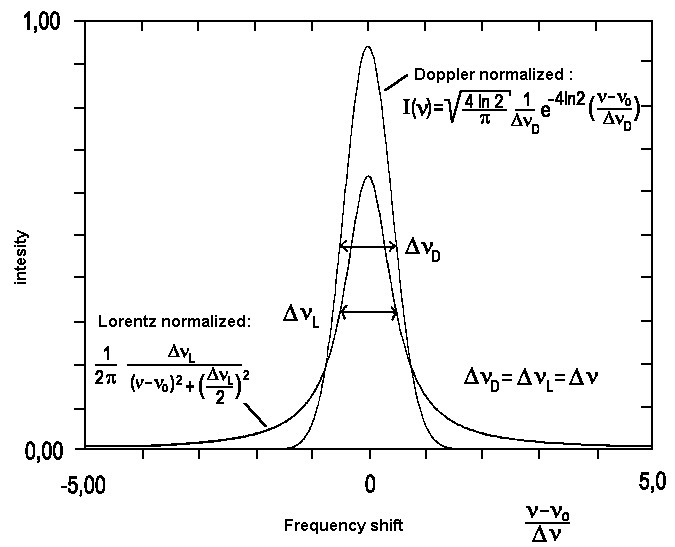
\includegraphics[width=(0.99\textwidth),height=(\textheight),keepaspectratio]{GLprofile}
\caption{Lorentzian vs Gaussian profile (in G manca un quadro all'esponente?!).}
\end{figure}


\end{usefull}

\clearpage

\subsubsection{Natural broadening (radiation damping)}

The motion of optical electron in a EM field of plane wave obey the (forced, damped) oscillation motion
\begin{equation*}
\ddot{x}+\gamma\dot{x}+\omega_0^2x=\frac{eE}{m}\cos{\omega t}
\end{equation*}

The oscillating (accelerating) charge radiate itself: the system losses energy.

Rate of energy radiation $P=\frac{2}{3}\frac{e^2\ddot{x}^2}{4\pi \epsilon_0c^3}$.

Classical absorption cross section
\begin{align*}
&a(\omega)=\frac{8\pi e^2}{3m_e^2c^4}[\frac{\omega^4}{(\omega^2-\omega_0^2)^2+\gamma^2\omega^2}]&\intertext{$\gamma$ is the classical damping constant}\\
&\gamma=(\frac{2e^2}{3m_ec^3})\omega_0^2
\end{align*}

Il principio di indeterminazione ci dice che un livello atomico non ha energia definita $E_i$ ma \'e una sovrapposizione di stati possibili attorno ad $E_i$: \mblock{\Delta \nu=\frac{\Delta E}{h}}. Transitions of electrons between levels doesn't correspond to specified energy difference.

Replace $\gamma$ with QM damping constant
\begin{align*}
&\Gamma_i=\sum_{l<i}A_{il}\\
&\Gamma_j=\sum_{l<j}A_{jl}
\end{align*}

\begin{definition}{Einstein coefficient $A_{ij}$}
The Einstein coefficient $A_{ij}$ is the probability in  unit of \si{\per\second} of a transition from upper level i to lower level j.
\end{definition}

The resulting profile for absorption cross section of a transition between two states reflects intrinsic energy width of both states: \mblock{\gamma_{nat}=\frac{\Delta E_i-\Delta E_f}{h/(2\pi)}}


\subsection{Absorption cross-section.}

Normalized absorption cross section for damping constant
\begin{align*}
&\phi_{\nu}=\frac{\frac{\Gamma}{4\pi^2}}{(\nu-\nu_0)^2+\frac{\Gamma^2}{(4\pi)^2}}\\
&\phi_{Max}=\phi_{\nu_0}=\frac{4}{\Gamma}\\
\end{align*}

For allowed transitions $\Delta\nu_{\frac{1}{2}}=\frac{\Gamma}{2\pi}\leq \SI{e-5}{\nano\meter}$ (FWHM), $\Delta\lambda=\frac{c}{\nu^2}\Delta\nu=\frac{2\pi}{3}\frac{e^2}{m_ec^2}\approx\SI{e-4}{\angstrom}$.

\subsection{Corpo nero}

L'energia irradiata per unit\'a di tempo per unit\'a di superficie nell'angolo solido $4\pi$ da un corpo nero di temperatura T
\begin{align*}
&(\int\,d\Omega I_{\nu}=)S_{\nu}=\frac{(4\pi)2 h\nu^3}{c^2}\frac{1}{\exp{\frac{h\nu}{KT}}-1}&\intu{nell'intervallo di frequenza $\nu,\nu+\,d\nu$, $\nu=\frac{c}{\lambda}$, $d\nu=-c\frac{d\lambda}{\lambda^2}$}\\
&(\int\,d\Omega I_{\lambda}=)S_{\lambda}=\frac{(4\pi)2 hc^2}{\lambda^5}\frac{1}{\exp{\frac{hc}{\lambda KT}}-1}&\intu{nell'intervallo di frequenza $\lambda,\lambda+\,d\lambda$}\\
&W=\sigma T^4&\intu{Legge di Stefan-Boltzmann}
\end{align*}

Il massimo di $S_{\lambda}$ segue la legge di Wien $\lambda_{Max}T=\const{}$.

\begin{definition}{Temperatura efficace}
\begin{equation*}
L=4\pi R^2\sigma T_e^4
\end{equation*}
\end{definition}

\begin{definition}{Temperatura di brillanza}
\begin{align*}
&I_{\nu}=B_{\nu}(T_b)\\
&L_{\lambda}=4\pi R^2\frac{2\pi hc^2}{\lambda^5}\frac{1}{\exp{\frac{hc}{\lambda KT_b}}-1}
\end{align*}
\end{definition}

Per il sole: $T_b(UV)\approx 5000\si{\kelvin}$, $T_b(V)\approx 6000\si{\kelvin}$

\begin{definition}{Temperatura di colore}
Temperature of a true blackbody is determined by intensity at two wavelength: match to shape of continous spectrum rather integrated power. 

\begin{equation*}
\frac{L_{\lambda_1}^O}{L_{\lambda_2}^O}=\frac{S_{\lambda_1}}{S_{\lambda_2}}
\end{equation*}

\end{definition}

\begin{definition}{Color index}
$B-V$ is defined by measurng luminisity with blue sensitive photographic plate (B) and with yellow-sensitive plate and yellow filter (V).
\end{definition}


\section{Righe dell'idrogeno.}

I livelli energetici dell'idrogeno sono \mblock{E_n=-\frac{\ER{}}{n^2},\ \ER{}\approx\SI{13.6}{\ev}}.

\begin{figure}[!ht]
\centering
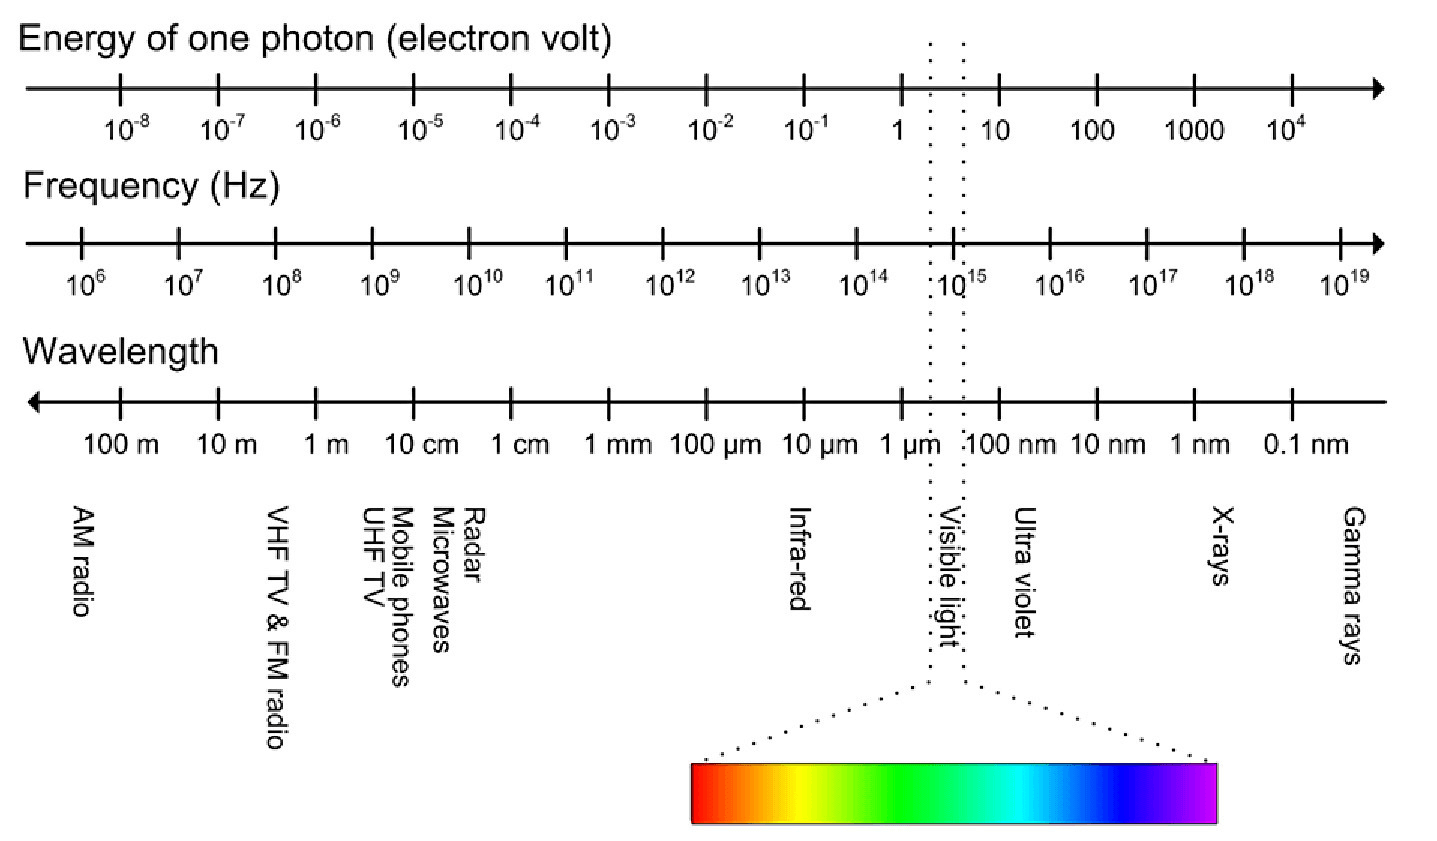
\includegraphics[width=(0.99\textwidth),height=(0.9\textheight),keepaspectratio]{PHevomega}
\caption{Spettro luminoso: energie, frequenze, regioni.}
\end{figure}

Le transizioni tra i livelli corrispondono a differenze di energie $E_{n,m}=\ER{}(\frac{1}{n^2}-\frac{1}{m^2})$
\begin{itemize}
    \item $n=1$: serie di Lyman (UV).
    \item $n=2$: serie di Balmer (V).
    \item $n=3$: serie di Paschen (IR).
\end{itemize}

\subsection{Popolazione dei livelli.}

A basse temperature H \'e neutro:
\begin{equation*}
    \frac{P(n)}{P(0)}\propto \exp{\frac{E_{0,n}}{KT}}
\end{equation*}
il rapporto \'e molto piccolo anche per $n=2$, primo eccitato.

A temperature intermedie (\SI{9520}{\kelvin}) la popolazione del primo eccitato $n=2$ raggiunge un massimo (stelle tipo spettrale A): le righe dell'idrogeno dominano lo spettro visibile.

\begin{figure}[!ht]
\centering
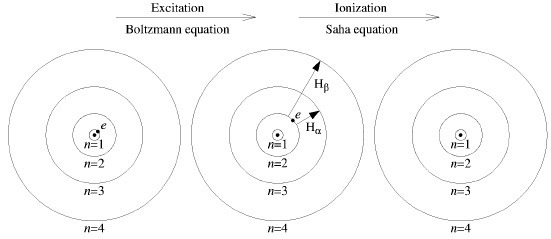
\includegraphics[width=(0.99\textwidth),height=(0.9\textheight),keepaspectratio]{boltzmansaha}
\caption{Determinazione popolazione livelli eccitati stati ionizzazione di H.}
\end{figure}

\begin{figure}[!ht]
\centering
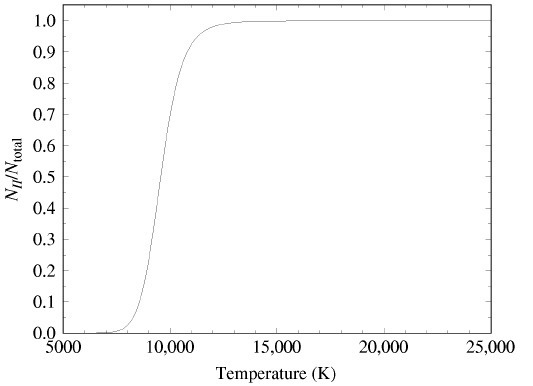
\includegraphics[width=(0.99\textwidth),height=(0.9\textheight),keepaspectratio]{HIIT}
\caption{Popolazione di HII.}
\end{figure}

\begin{figure}[!ht]
\centering
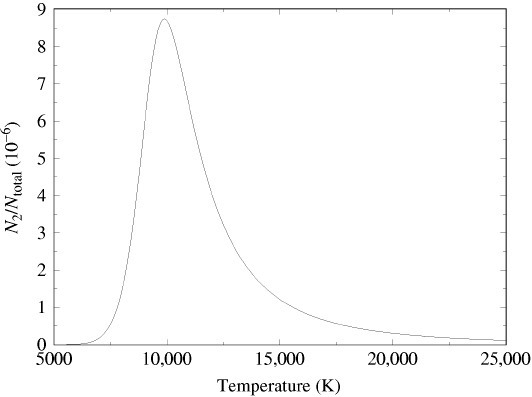
\includegraphics[width=(0.99\textwidth),height=(0.9\textheight),keepaspectratio]{HIn2pop}
\caption{Popolazione del livello primo eccitato di HI.}
\end{figure}

\clearpage

\section{Allargamento delle righe spettrali.}

\subsection{Allargamento (thermal) Doppler (GP)}

Lungo la linea di vista gli atomi hanno una distribuzione di velocit\'a gaussiana (moti termici e turbolenti)
\begin{align*}
&dn(v_e)\propto\exp{-\frac{v_e^2}{\alpha}}\,dv_e\\
&\alpha=\frac{2KT}{m}+v_{turb}^2
\end{align*}

La riga corrisponde ad una lunghezza d'onda diversa con
\begin{equation*}
\Delta\lambda\approx\frac{v_e}{c}\lambda
\end{equation*}

Per l'insieme degli atomi avremo una distribuzione di frequenze proprie

\begin{equation*}
\sigma(\nu)\propto\int\,d\nu*\exp{-A(\nu*-\nu_0)^2}\frac{1}{(\nu-\nu*)^2+(\frac{\gamma}{4\pi})^2}
\end{equation*}

Il profilo della riga \'e caratterizzato dalla curva pi\'u larga: Lorenziana, parametrizzata dalla larhezza naturale o gaussiana dalla distribuzione di velocit\'a.

Fatti:
\begin{itemize}
    \item Per il sole la gaussiana \'e pi\'u larga della lorenziana di un fattore \num{e3}.
\end{itemize}


\subsection{Allargamento da pressione (LP)}

La vicinanza di altre particelle perturba i livelli atomici (atmosfere con alta pressione): la condizione di equilibrio idrostatico in termini di profondit\'a ottica $\TDy{\tau}{P}=\frac{g}{\kappa}$ dice che nella regione $\tau\approx1$ la pressione $P_{Atm}\approx\frac{g}{\kappa}$, dove g \'e l'accelerazione di gravit\'a che determina l'allargamento da pressione mentre l'opacit\'a $\kappa$ varia meno rispetto a g.

Fatti:
\begin{itemize}
    \item La dominanza dell'allargamento da pressione nelle stelle di sequenza (nane) permette la classificazione empirica in classi di luminosit\'a.
\end{itemize}


\subsection{Allargamento quasi-statico.}

Effetto del campo esterno sull'atomo: perturba i livelli e cambia le energie di transizione. Distribuzione statistica nello spazio-tempo: distribuzione delle energie.

\mblock{\Delta t_{int}>\Delta T_{em}\approx\SI{e-9}{\second}}: nearby particles shift energy levels of emitting particle.

La larghezza \'e funzione soprattutto di $\rho$ (meno di $T$): si ha una dipendenza del tipo \mblock{\gamma\propto\exv{r}\expy{-n}}, con
\begin{itemize}
    \item Stark effect (WD): $n=3$.
    \item Van der Waals force (cool stars): $n=6$.
    \item Dipolar coupling between particles of same species: $n=3$.
\end{itemize}

\subsection{Allargamento da impatto (LP)}

Da un punto di vista semi-classico durante una collisione si interrompe l'assorbimento alla frequenza di transizione dell'atomo.

\mblock{\Delta t_{col}<\Delta T_{em}\approx\SI{e-9}{\second}}, funzione di $(T,\rho)$

\subsection{Allargamento dovuto alla rotazione.}

Ho un effetto Doppler di segno opposto nell zone simmetriche rispetto all'asse della superficie
\begin{equation*}
    \frac{\Delta\lambda}{\lambda}\approx\frac{\Delta v}{c}\approx2\frac{\omega R}{c}
\end{equation*}

Fatti:
\begin{itemize}
    \item Stelle rapidamente rotanti (A,O,B).
    \mblock{\omega R\approx v_F=\sqrt{\frac{2GM}{R}}\approx\SI{e3}{\kilo\meter\per\second}} e \mblock{\frac{\Delta\lambda}{\lambda}\approx\num{e-3}}: nel visibile $\Delta\lambda\approx\SI{10}{\angstrom}$.
    \item Le classi O,B sono rotatori veloci, il tipo A comprende rotatori lenti e veloci e $Ap$, i tipi spettrali pi\'u freddi da F in poi sono rotatori lenti.
\end{itemize}


\section{Astro-spettroscopia.}

\subsubsection{Spectral resolution.}

A varie dispersioni sul ricevitore gli spettri ci danno informazioni diversi
\begin{itemize}
    \item Bassa dispersione: \SI{e2}{\angstrom\per\milli\meter}.
    
    Tipo spettrale.
    
    \item Media dispersione: \numrange{10}{100}\si{\angstrom\per\milli\meter}.
        
    Velocit\'a radiale, allargamento righe: P,T, righe peculiari.
        
    \item Alta dispersione: $\leq$\SI{10}{\angstrom\per\milli\meter}.
    
    $W_{\lambda}(\eta_{\lambda})$: analisi quantitativa,  ricostruzione dell'atmosfera.

\end{itemize}


\subsubsection{Moto radiale.}

Le righe sono spostate verso il rosso/blu
\begin{align*}
    &\frac{\Delta\lambda}{\lambda}=z\approx\frac{v}{c}&\intu{small $v$}\\
    &1+z=\gamma(1+\frac{v_{\parallel}}{c})\\
    &v_{los}=c\exv{\frac{\Delta\lambda}{\lambda}}_{Righe}
\end{align*}

Classi di osservazioni:
\begin{itemize}
    \item Binarie spettroscopiche
    \item Stelle pulsanti
    \item Legge di Hubble: $v_{rad}\approx c$
\end{itemize}

\subsection{Gravitational red-shift}

Per oggetti densi \'e osservabile uno spastamento Doppler delle righe di assorbimento dovuto alla differenza tra energia gravitazionale sulla superficie della stella ed energia al punto d'osservazione:
\begin{align*}
&V_{grav}=\frac{GM}{Rc}\\
&\frac{\Delta\lambda}{\lambda}=\frac{E}{\Delta E}\overset{?}{=}\frac{Rc^2}{GM}
\end{align*}

\section{Classificazione degli spettri stellari}

In un grafico $U-B$ vs $B-V$ una successione di corpi neri di temperatura variabile \'e approssimativamente una linea retta.

\begin{figure}[!ht]
\centering
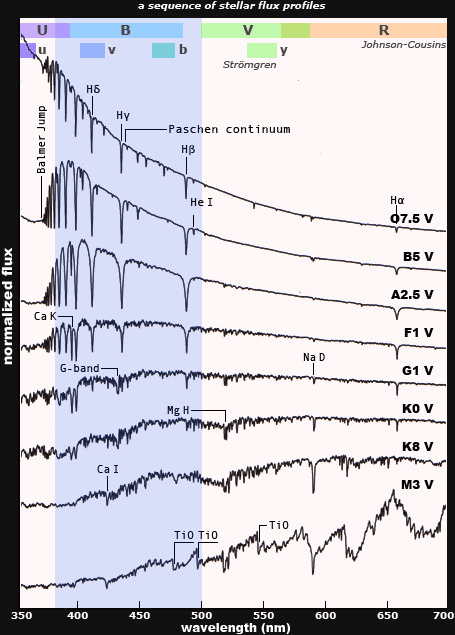
\includegraphics[width=(0.99\textwidth),height=0.9\textheight,keepaspectratio]{sequenceFP}
\caption{Sequence stellar flux profile.}
\end{figure}

La classificazione stellare consiste di una lettera per il tipo, numero per il sottotipo e un numero romano per la classe di luminosit\'a (I supergiganti, III giganti, IV subgiganti, V nane). Il tipo spettrale \'e individuato dalla distribuzione del continuo e dalla presenza di alcune righe.

La classe di luminosit\'a \'e individuata dalle caratteristiche delle righe: Larghezza/pressione supericiale.

\begin{figure}[!ht]
\centering
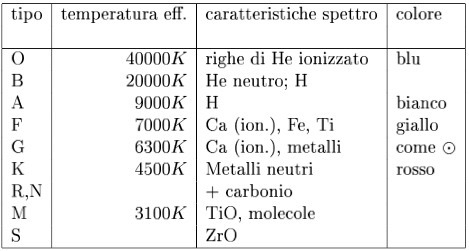
\includegraphics[width=(0.8\textwidth),height=(\textheight-11mm),keepaspectratio]{types}
\caption{Star types.}
\end{figure}

Fatti:
\begin{itemize}
\item O stars (\SI{30000}{\kelvin}): hottest stars, continuum strong in UV.

Strong He II lines in absorption, sometimes with few lines; He II dominates emission; He I lines weak but increasing in strength
from O5 to O9; hydrogen Balmer lines prominent but
weak relative to later types; lines of Si IV, O III, NIII
and C IV.

\item B stars (\SI{20000}{\kelvin}).

He I lines dominate, with maximum strength at B2; He I dominates He II lines virtually absent; hydrogen lines strengthening
from B0 to B9; Mg II and Si II lines

\item A stars (\SI{10000}{\kelvin}). 

Hydrogen lines reach maximum strength at A0; hydrogen Balmer lines dominate of ionised metals (Fe II, Si II, Mg II) at maximum strength near A5; Ca II lines strengthening; lines of neutral
metals appearing weakly.

\item F stars (\SI{7000}{\kelvin}).

Hydrogen lines weakening rapidly while H and K lines of CaII strengthen; neutral metal (Fe I and Cr I) lines gaining on ionised metal lines by large F

\item G stars (\SI{6000}{\kelvin}).

Hydrogen lines very weak; Ca II H and K lines reach maximum strength near G2; neutral metal (Fe I, Mn I,Ca I) lines strengthening while ionised metal lines
diminish; molecular G band of CH becomes strong.

\item Il sole \'e una stella di tipo G2.

\item K stars (\SI{4000}{\kelvin}).

Hydrogen lines almost gone; Ca lines strong; neutral metal lines very prominent; molecular bands of TiO begin (K2)
to appear by late K.

\item M stars (\SI{3000}{\kelvin}).

Neutral metal lines very strong; molecular bands prominent with TiO bands dominating by M5; vanadium oxide bands appear.

\end{itemize}


\begin{figure}[!ht]
\centering
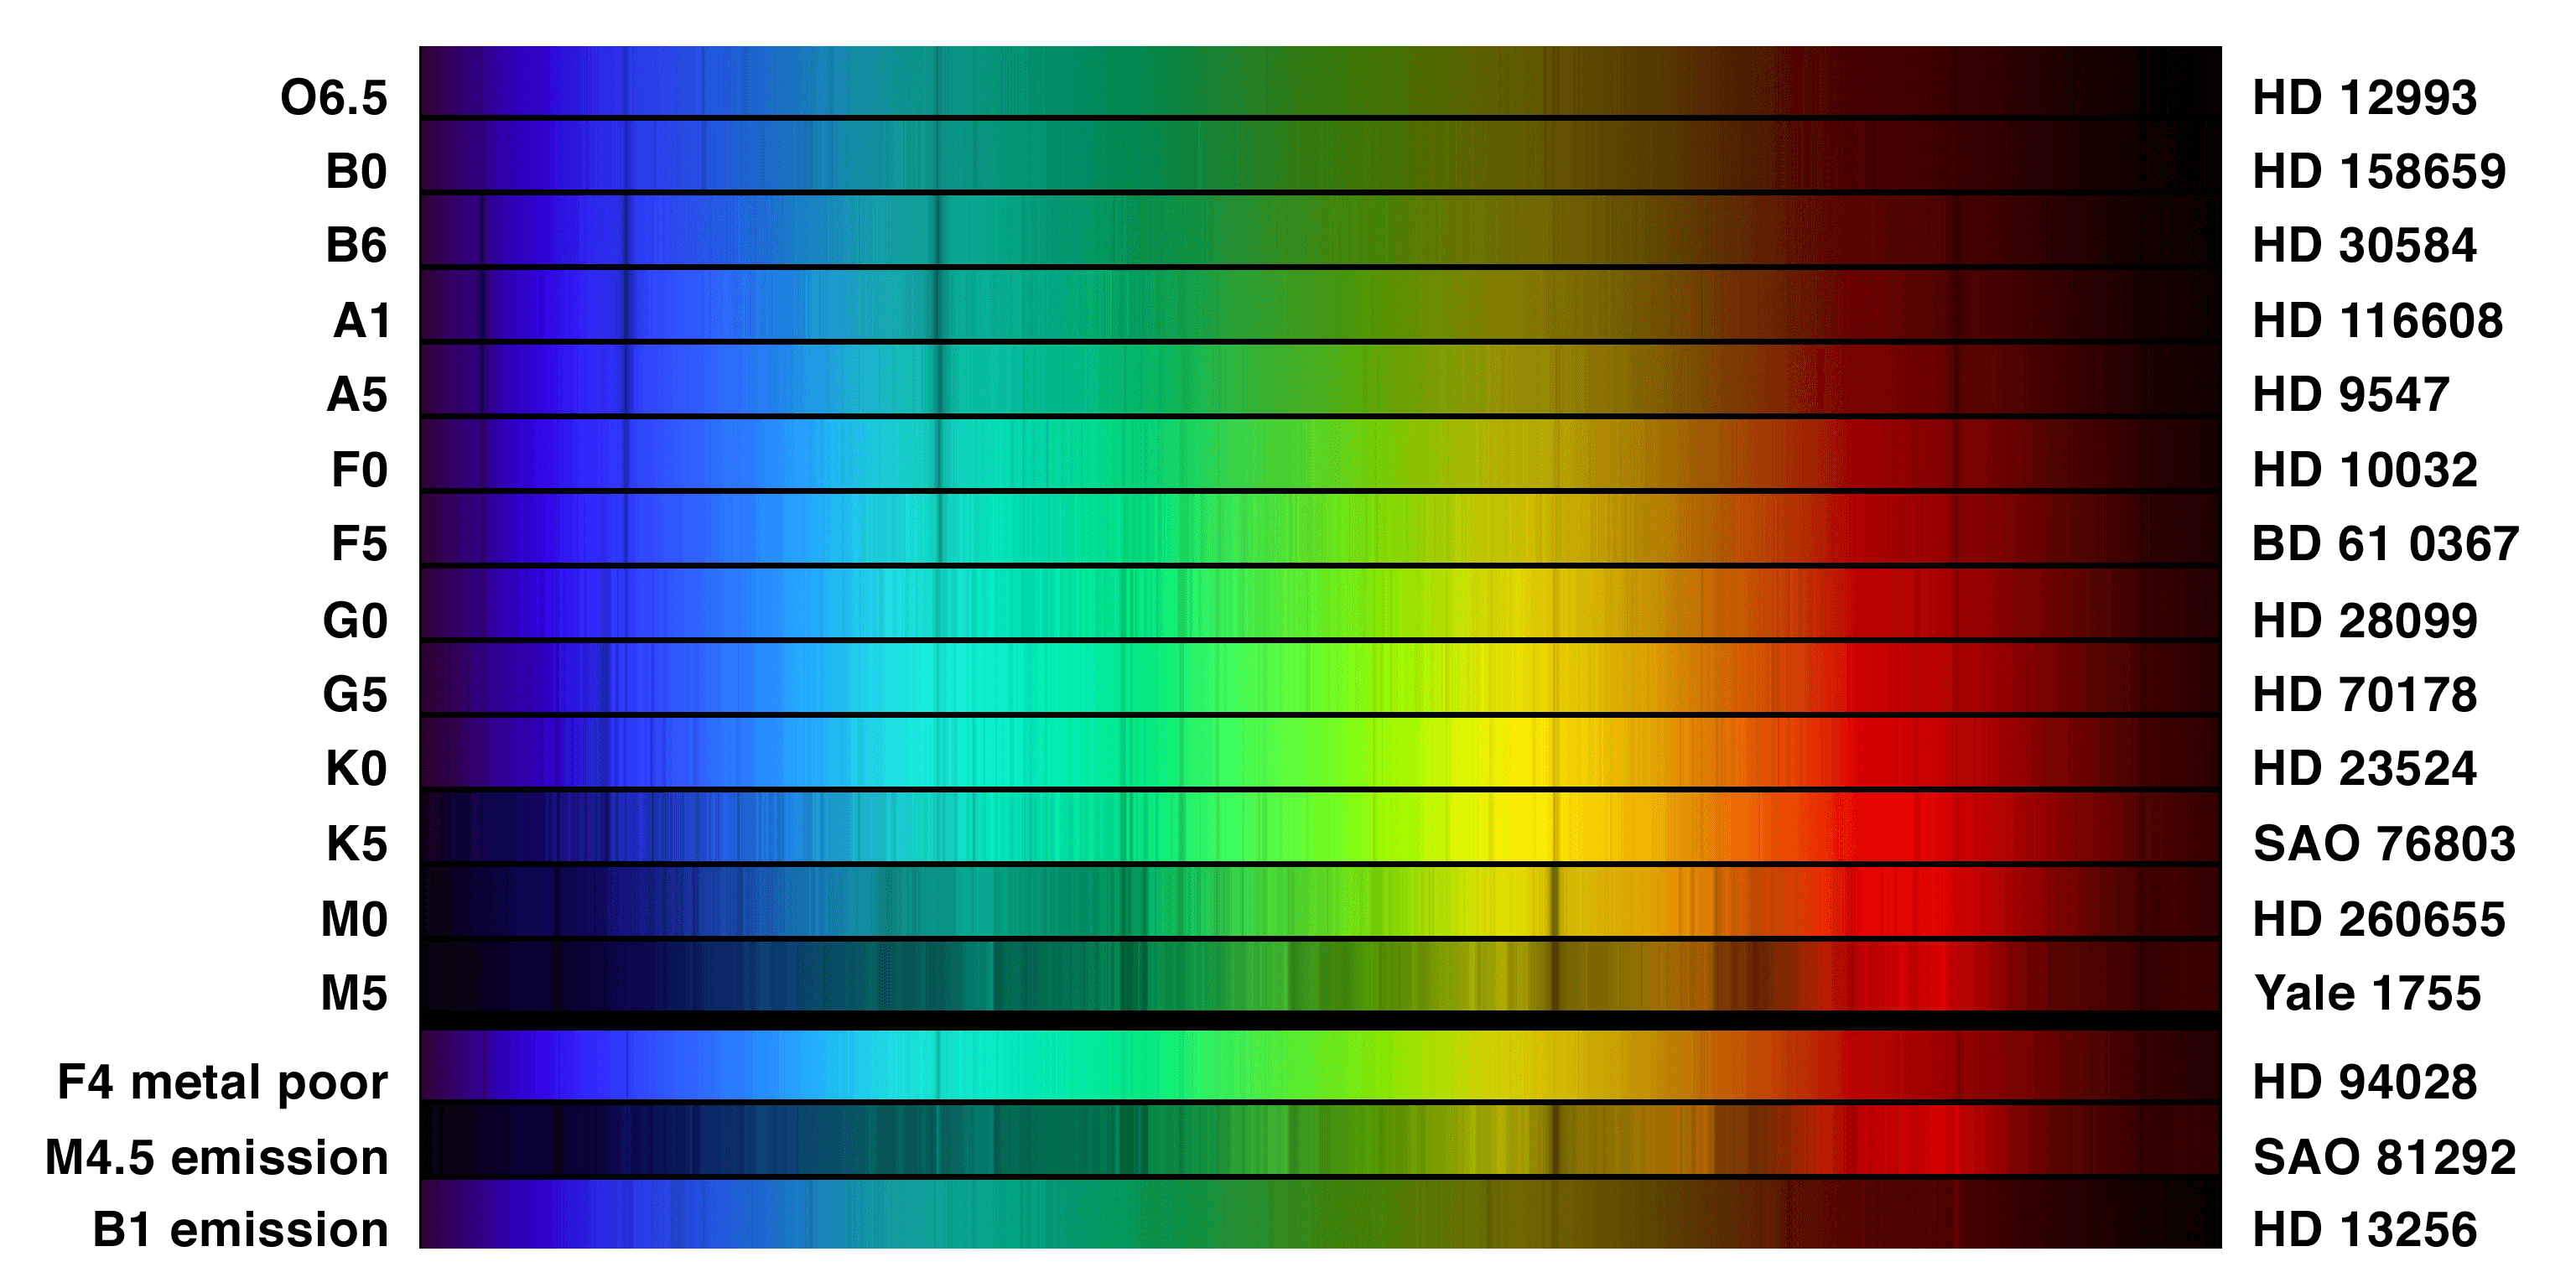
\includegraphics[width=(0.99\textwidth),height=\textheight,keepaspectratio]{spectral}
\caption{Spectral types.}
\end{figure}

\begin{figure}[!ht]
\centering
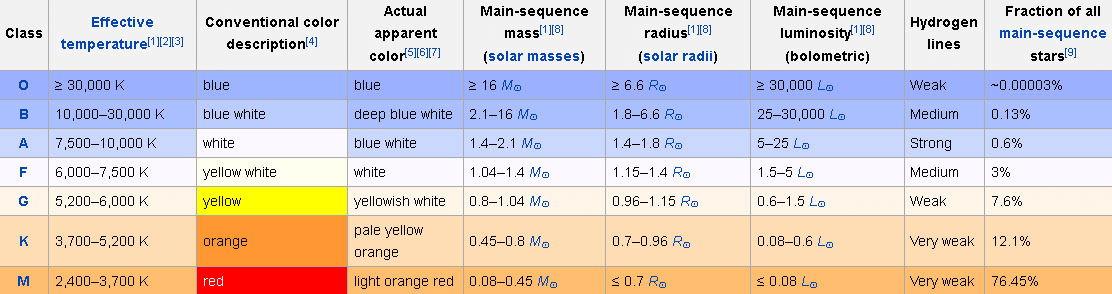
\includegraphics[width=(\textwidth),height=(\textheight-11mm),keepaspectratio]{classprop}
\caption{Classi stellari.}
\end{figure}

\clearpage



\chapter{Relazioni massa/luminosit\'a. Diagramma di \hr{}.}
\PartialToc

\subsection{Massa-Luminosit\'a}

\begin{usefull}{Massa-Luminosit\'a (relazione).}
\begin{align*}
    &\frac{L}{\lsun{}}\approx0.23(\frac{M}{\msun{}})\expy{2.3},\ (M<0.43\msun{})\\
    &\frac{L}{\lsun{}}\approx(\frac{M}{\msun{}})^4,\ (0.43\msun{}<M<2\msun{})\\
    &\frac{L}{\lsun{}}\approx1.5(\frac{M}{\msun{}})\expy{3.5},\ (2\msun<m<20\msun{})\\
    &\frac{L}{\lsun{}}\approx3200\frac{M}{\msun{}},\ (m>20\msun{})
\end{align*}
\end{usefull}



\section{Importanti relazioni semi-empiriche.}

\subsection{Massa-Luminosit\'a}

\begin{equation*}
    (\frac{L}{\lsun{}})=(\frac{M}{\msun{}})\expy{\frac{1}{4}}
\end{equation*}

\begin{todo}{Importanti relazioni semi-empiriche.}
clay pg 470-472.
$\S 1.6$ stellar interior
\end{todo}

\section{Diagrammi di HR: magnitudine vs colore.}


Considero il diagramma $M_V$ vs $(B-V)$ o $M_{B}$ vs spectral type (per stelle vicine) (\mblock{M_B=-2.5\log{\frac{L}{\lsun{}}}+4.72})

\subsection{Diagramma di HR per stelle vicine.}

\begin{figure}[!ht]
\centering
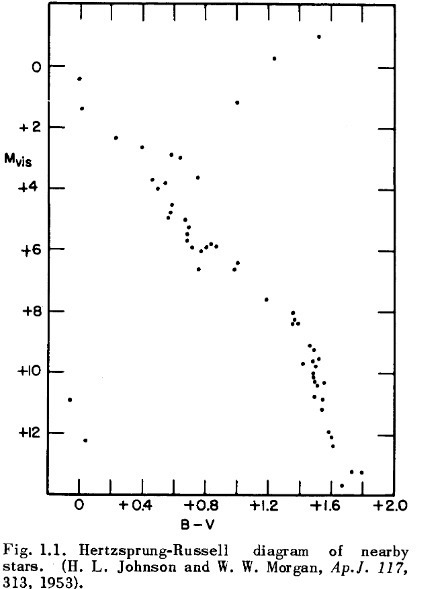
\includegraphics[width=(\textwidth),height=(0.8\textheight),keepaspectratio]{nearbyHR}
\caption{Diagramma HR di stelle vicine.}
\end{figure}

\clearpage

\subsection{Diagramma di HR per associazioni di stelle.}

Considero il diagramma di HR per associazioni fisiche di stelle.


La struttura di una stella \'e univocamente definita da massa, composizione chimica iniziale ed et\'a: un diagramma di ammasso si pu\'o vedere come una sequenza di stelle con massa variabile e stessa composizione iniziale ed et\'a.

\begin{figure}[!ht]
\centering
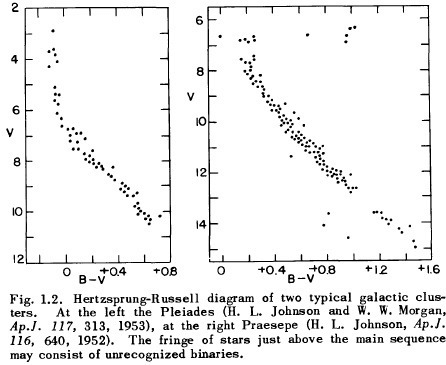
\includegraphics[width=(\textwidth),height=(\textheight-11mm),keepaspectratio]{GCHR}
\caption{Diagramma di HR di un cluster.}
\end{figure}


\begin{figure}[!ht]
\centering
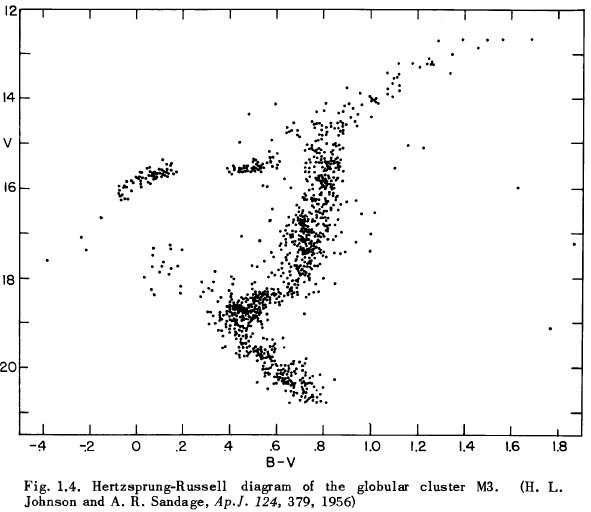
\includegraphics[width=(\textwidth),height=(\textheight-11mm),keepaspectratio]{GlobularCHR}
\caption{Diagramma di HR di un ammasso globulare.}
\end{figure}

\clearpage

\subsection{Evolution of a cluster of stars.}

\subsubsection{Evolution from main sequence.}

Il processo di fusione $4H\to He$ produce \SI{6.4e18}{\erg\per\gram}.

Suppongo che una stella di massa M si allontani dalla sequenza principale quando ha costituito un core di He di massa $fM$:

se $X_H$ \'e la frazione di H in massa originaria si deve convertire in He una massa $fX_HM$ di H quindi l'energia irradiata \'e $E=fX_HM(\num{6.4e18})=\num{1.3e52}fX_H\frac{M}{\msun{}}\si{\erg}$.

La vita di sequenza principale pu\'o essere stimata
\begin{equation*}
    \tau_E=\frac{E}{L}=\num{1.1e11}fX_H\frac{M/\msun{}}{L/\lsun{}}\si{\year}
\end{equation*}

Fatti:
\begin{itemize}
    \item Per stella solar-like $f=15\%$: using M/L relatioship
    \begin{equation*}
    \tau_E=\num{12e9}(\frac{L}{\lsun{}})\expy{-\frac{3}{4}}\si{\year}
    \end{equation*}
    \item Posso approssimare l'et\'a di un ammasso con l'et\'a delle sue stelle pi\'u luminose. 
\end{itemize}

Ad alta luminosit\'a la linea della sequenza principale svolta a destra.

\subsubsection{Turn-off: ramo delle giganti.}

Una classificazione dei diagrammi in sequenze di $(B-V)_{\text{Turn-off}}$ crescenti corrisponde ad una sequenza di et\'a: turn-off blue per ammasso giovane, turn-off giallo ammasso vecchio.


\begin{figure}[!ht]
\centering
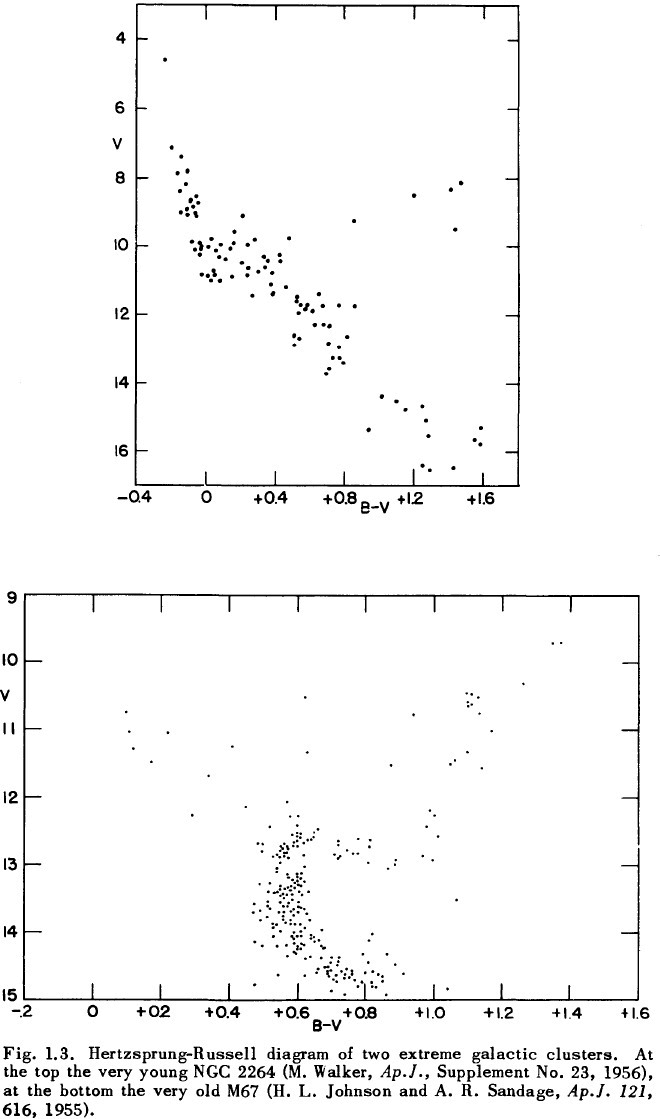
\includegraphics[width=(\textwidth),height=(0.9\textheight),keepaspectratio]{extremeGCHR}
\caption{Diagramma di HR di cluster giovane (in alto) vecchio (in basso).}
\end{figure}

\clearpage

\section{Caratteristiche delle stelle nelle zone del diagramma di HR.}

\begin{figure}[!ht]
\centering
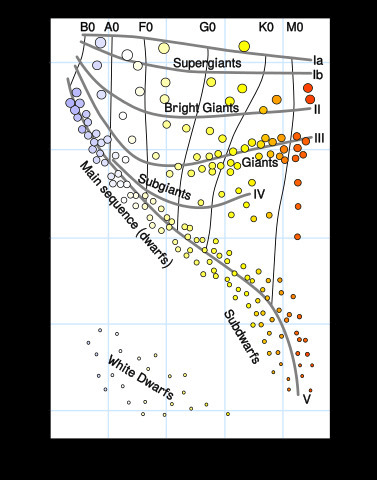
\includegraphics[width=(\textwidth),height=(0.9\textheight),keepaspectratio]{HRpizza}
\caption{Diagramma di HR: MS, WD, SD, giant branch.}
\end{figure}

\subsection{Passaggio al diagramma raggio-Luminosit\'a.}

Passo alla rappresentazione con in ordinata L e in ascissa $T_e$:

\begin{align*}
    &\log{\frac{L}{\lsun{}}}=\frac{1}{2.5}(M_{B\odot}-M_B)\\
    &=4\log{\frac{T_e}{T_{e\odot}}}+2\log{\frac{R}{\rsun}}
\end{align*}

\begin{figure}[!ht]
\centering
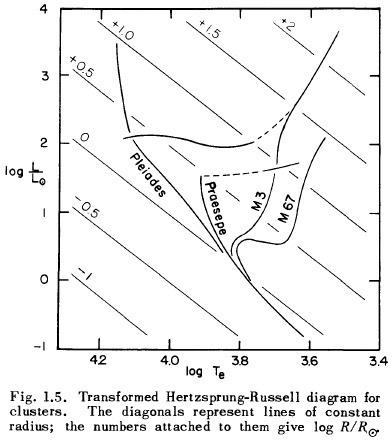
\includegraphics[width=(\textwidth),height=(\textheight-11mm),keepaspectratio]{CsHR}
\caption{Diagramma HR $L$ vs $T_e$.}
\end{figure}

\clearpage

\subsection{Nane.}



\subsection{Sub-nane.}

Caratteristiche:
\begin{itemize}
    \item Deboli righe di assorbimento.
    \item Parallela alla MS circa 1 magnitudine superiore.
    \item Per pari $T_e$ $\log{\frac{L_{SN}}{L_{MS}}}=-0.4$.
\end{itemize}

Le differenze di luminosit\'a e di caratteristiche spettrali sono attribuibili alla diversa composizione chimica.

Fatti:
\begin{itemize}
    \item La sequenza principale degli ammassi globulari coincide con quella delle sub-nane.
\end{itemize}

\subsection{Nane bianche.}

Caratteristiche:
\begin{itemize}
    \item Alta densit\'a superficiale: righe allargate.
    \item Raggio quasi costante circa $\frac{1}{100}\rsun{}$.
    \item Oggetti estremamente densi.
    \item Fase finale evoluzione stellare.
\end{itemize}


\section{Popolazioni stellari.}

Fatti:
\begin{itemize}
\item Existence in late F early G stars of strong-line and weak-line with different kinematical properties: generally the strong lines have low velocity, the weak line higher velocity.
\end{itemize}

\begin{figure}[!ht]
\centering
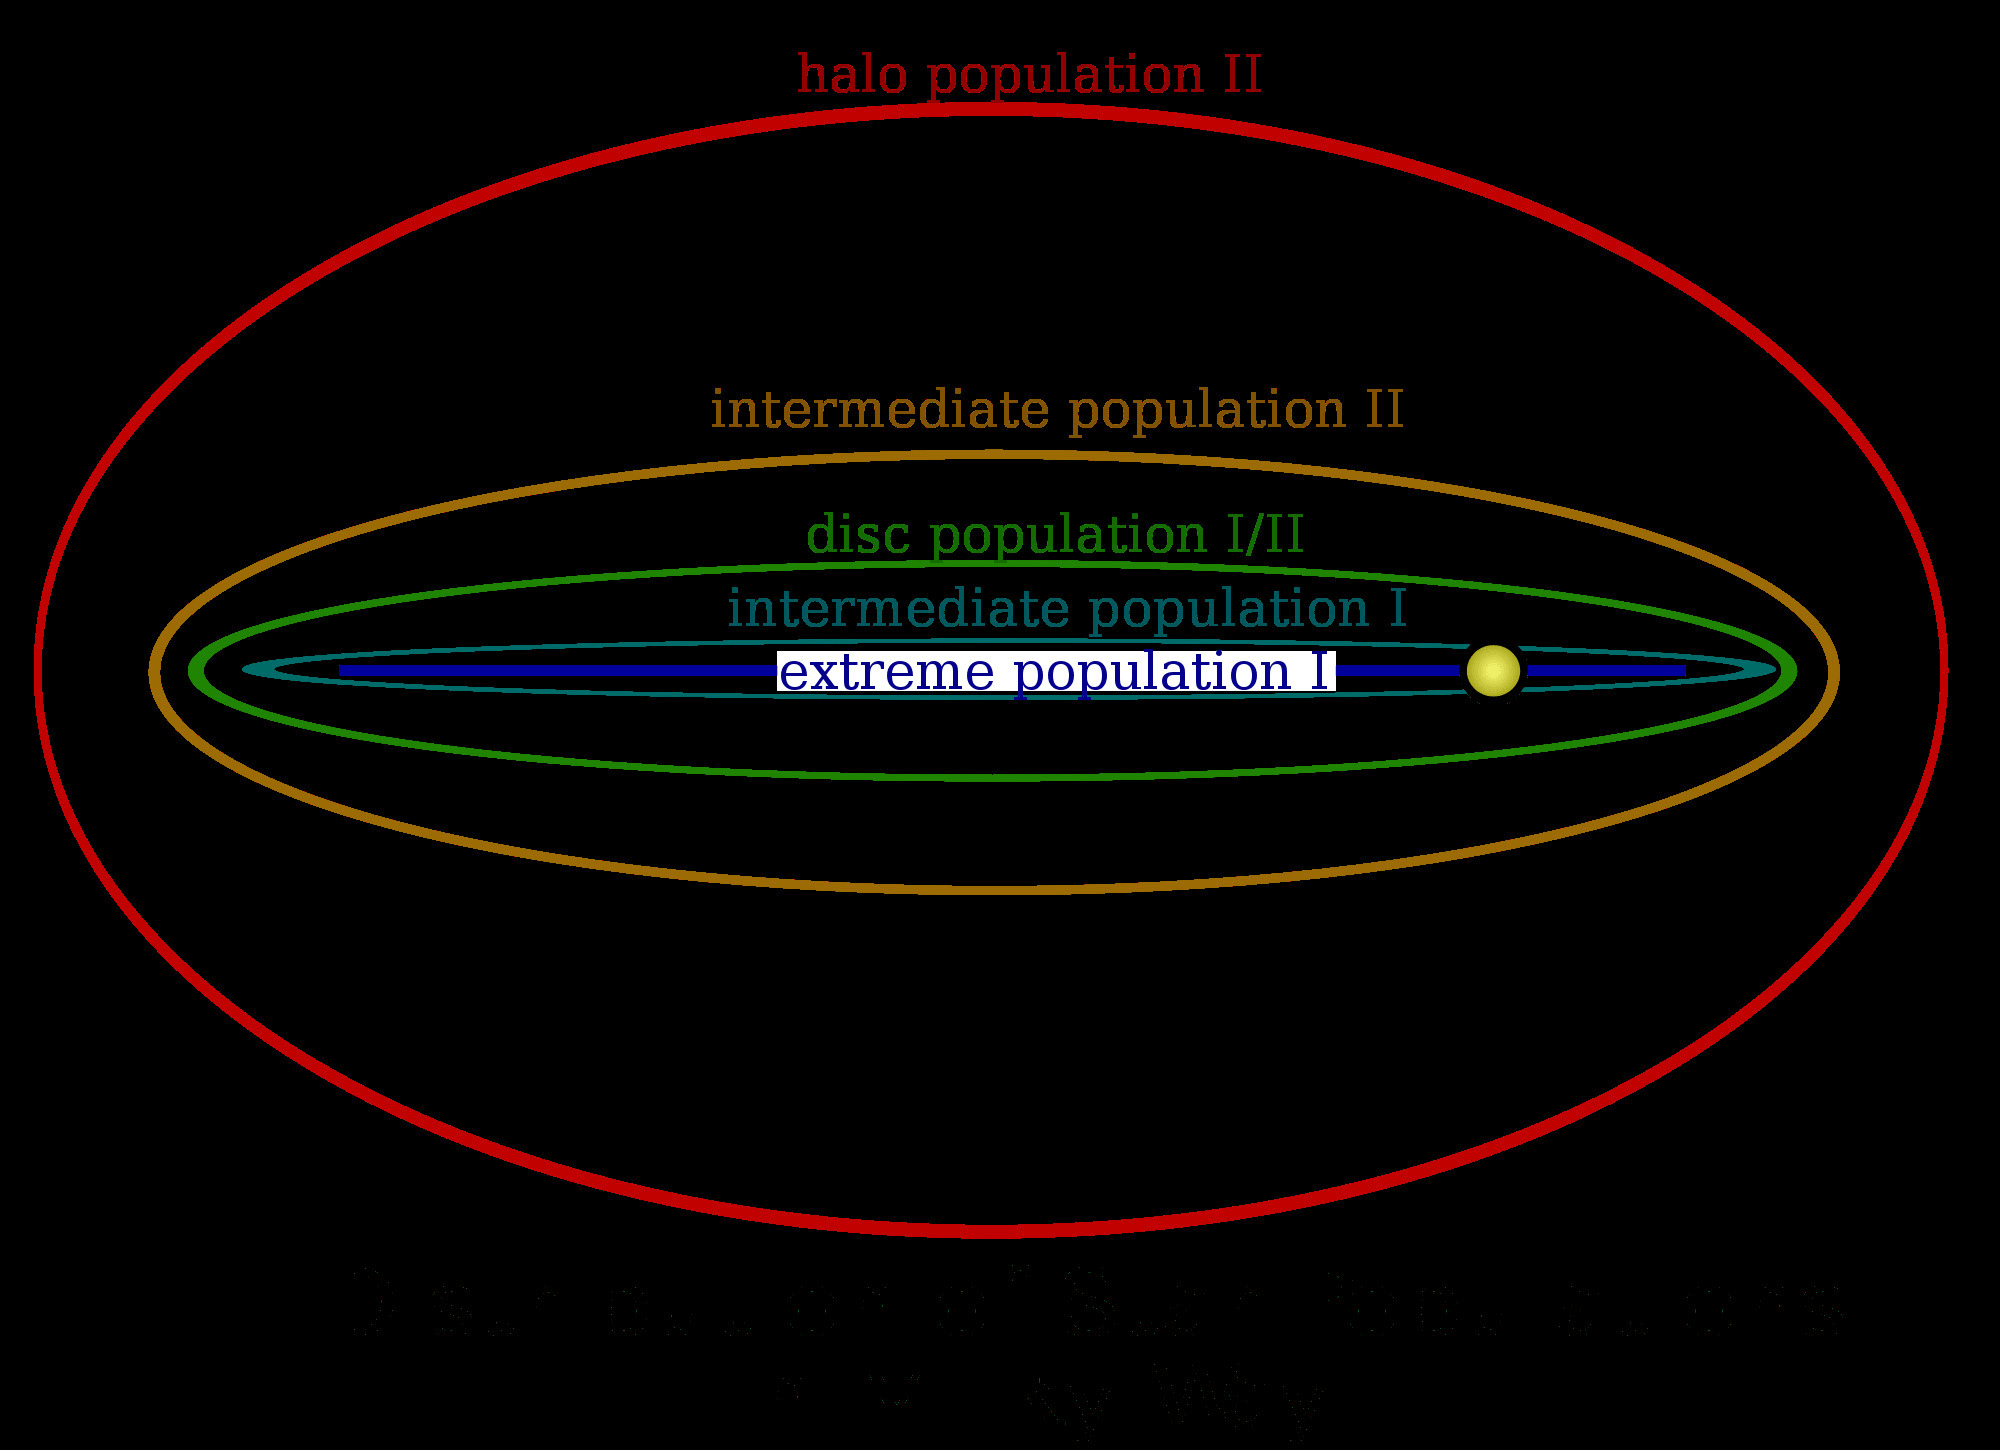
\includegraphics[width=(\textwidth),height=(\textheight-11mm),keepaspectratio]{Starpop}
\caption{Popolazioni stellari: distribuzione galattica.}
\end{figure}

\begin{figure}[!ht]
\centering
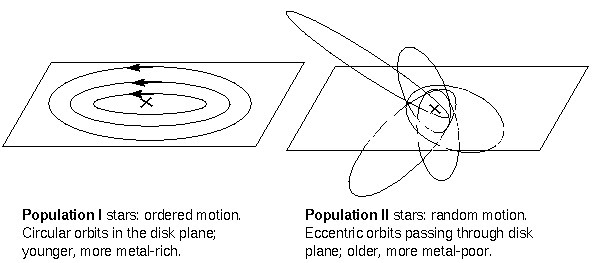
\includegraphics[width=(\textwidth),height=(\textheight-11mm),keepaspectratio]{starpops}
\caption{Popolazioni stellari: differenze orbitali.}
\end{figure}

\subsection{Cluster di stelle.}

\begin{definition}{Star cluster.}
Is a group of stars that have a much stronger gravitational attraction to each others than to general field of stars.
\end{definition}

\subsubsection{Globular cluster.}



\begin{itemize}
    \item Number of stars: approx. \num{e5}.
    \item Far from the Sun: magnitude of RR Lyra stars.
    \item Location: Corona or galactic nucleus.
    \item Diameter of high density region approx \SI{10}{\parsec}, density \SI{e3}{\per\parsec}.
    \item Diameter \numrange{50}{100} \si{\parsec}.
    \item Color of the brightest: red.
    \item Densit\'a di stelle (\si{\cubic\parsec}): \numrange{0.5}{e3}.
    \item Nomi: M3
\end{itemize}

\subsubsection{ Open Cluster (Galactic cluster).}

\begin{itemize}
    \item Few-thousands stars randomly distributed.
    \item Found in galactic disc.
    \item Location: disk.
    \item Number of stars: \numrange{50}{e3}.
    \item Color of the brightest: red/blue.
      \item Densit\'a di stelle (\si{\cubic\parsec}): \numrange{0.1}{10}.
    \item Nomi: Hyades, Pleiades.
\end{itemize}

\subsubsection{Association.}

Open cluster containing most luminous main sequence stars of type $O/B$. O stars are not randomly distributed: O/B/WR are scattered in a region of \SI{100}{\parsec}.

\begin{itemize}
    \item Location: spiral harms.
    \item Diameter: \numrange{30}{200}\si{\parsec}
    \item Number of stars \numrange{10}{100}?
    \item Color of the brightest: blue.
      \item Densit\'a di stelle (\si{\cubic\parsec}): \num{0.01}.
    \item Nomi: Orion.
\end{itemize}
    


Fatti:
\begin{itemize}
    \item Le supergiganti blu sono stelle giovani vicine a nubi interstellari.
    \item Espansione di ammassi/associazioni contenenti SG blue permette, ricostruendo all'indietro il loro moto, di limitare superiormente la loro et\'a a \SI{e8}{\year}.
    \item Le galassie ellittiche e gli ammassi globulari appaiono prive di gas interstellare e polvere (Highly stable dynamical system).
\end{itemize}


\subsection{Comportamento cinematico}

\'E possibile separare le stelle vicine in due gruppi:
\begin{itemize}
    \item Alta velocit\'a sul piano galattico.
    
    Giganti rosse (HR simile agli ammassi globulari), subnane, 
    
    \item Bassa velocit\'a sul piano galattico.
    
    Stelle di tipo O/B (HR simile ad ammassi galattici), nubi interstellari.
\end{itemize}

Fatti:
\begin{itemize}
    \item Gli ammassi galattici presentano moto d'insieme di moderata velocit\'a a differenza degli ammassi globulari.
    \item Ad alta velocit\'a sul piano galattico corrisponde alta velocit\'a ortogonale: configurazione sempre pi\'u sferica.
    \item Le stelle ad alta veloci\'a hanno un moto retrogrado sul piano galattico (alone esterno).
\end{itemize}

\subsection{Evoluzione della galassia.}

Trasformazione di una struttura quasi-sferica ad un disco accompagnato da un rarefatto alone.

\begin{todo}{High/low velocity galactic plane}
Moto retrogrado
\end{todo}


\subsubsection{Popolazione I.}

Si distinguono spettroscopicamente stelle con righe forti (lente) e stelle con righe deboli (veloci).

\begin{itemize}
    \item (Young) extreme pop I.
    
    Typical member: Blue giant, variabili T Tauri, Cefeidi.
    
    Where: ammassi aperti, galactic cluster, braccia a spirale, G (spirale, irregolare).
    
    AVG velocity: \SI{8}{\kilo\meter\per\second}. Shape of subsystem: flat. Distanza dal PG: \SI{60}{\parsec}.
    
    Metallicit\'a: $\frac{Z}{Z_{\odot}}>1$.
    
    Et\'a (risp. universo): \numrange{0}{0.005}.
    
    \item (Int.) Pop I. 
    
    Typical member: Stelle a forti righe metalliche, Supernovae II, vicine del Sole.
    
    AVG velocity: \SI{10}{\kilo\meter\per\second}.
    
    Distanza dal piano galattico: \SI{160}{\parsec}.
    
    Metallicit\'a: $\frac{Z}{Z_{\odot}}>0.75$.
    
    Et\'a (risp. universo): \numrange{0.05}{0.25}.
    
    Where: Disco.
    
    \item (Old/disc) Pop I. 
    
    Typical member: Stelle a deboli righe metalliche, novae,nebulase planetarie, RR Lyrae, Periodic ($P<0^d.4$).
    
    AVG velocity: \SI{16}{\kilo\meter\per\second}. Distanza dal piano galattico: \SI{300}{\parsec}.
    
    Metallicit\'a: $\frac{Z}{Z_{\odot}}>0.5$.
    
    Et\'a (risp. universo): \numrange{0.25}{0.8}.
    
    Where: Disco, nucleo galattico (Bulges).

\end{itemize}

\subsubsection{Popolazione II.}

Si distinguono ammassi globulari e stelle ad alta velocit\'a.

\begin{itemize}
    \item Intermediate Pop. II:
    
    Stelle: Stelle ad alta velocit\'a, variabili a lungo periodo, RR Lyrae.
    
    AVG velocity(ortogonale al piano galattico): \SI{25}{\kilo\meter\per\second}.
    
    Where: Galassie ellittiche, disco spesso, ammasso globulare.
    
    Distanza dal piano galattico: \SI{500}{\parsec}.
    
    Metallicit\'a: $\frac{Z}{Z_{\odot}}=0.25$.

    Et\'a in et\'a dell'universo: \numrange{0.8}{1}.

    \item Pop II di Bulge:
    
    Where: Nucleo galattico.
    
    Stelle: Nebulose planetarie, Cefeidi.
    
    Metallicit\'a: $\frac{Z}{Z_{\odot}}=\numrange{0.1}{2.}$.
    
    Et\'a in et\'a dell'universo: \numrange{0.5}{1}.
    
    \item Extreme (halo) Pop. II:
    
    Stelle: Bright red giants, globular cluster, subdwarf, RR Lyrae $\Pi>0^d.4$, ramo orizzontale HR.
    
    AVG velocity(ortogonale al piano galattico): \SI{75}{\kilo\meter\per\second}.
    
    Where: Ammassi globulari, galassie ellittiche.
    
    Distanza dal piano galattico: \SI{2000}{\parsec}.
    
    Metallicit\'a: $\frac{Z}{Z_{\odot}}=\numrange{0.03}{0.1}$.

    Et\'a in et\'a dell'universo: \numrange{0.9}{1}.

    \item Pop II di Bulge:
    
    Where: Nucleo galattico.
    
    Stelle: Nebulose planetarie, Cefeidi.
    
    Metallicit\'a: $\frac{Z}{Z_{\odot}}=\numrange{0.1}{2.}$.
    
    Et\'a in et\'a dell'universo: \numrange{0.5}{1}.
\end{itemize}





\part{Descrizione semi-quantitativa dell'universo.}
%\chapter{Sistemi planetari.}
\PartialToc

\section{Classificazione.}

\subsection{Definizione pianeta (IAU).}

Un pianeta ha le seguenti caratteristiche
\begin{itemize}
    \item \'E in orbita attorno ad una stella di riferimento.
    \item \'E abbastanza massiccio da essere dominato dalle forze di gravit\'a: forma di equilibrio ''idrostatica''.
    \item Ha completamente ripulito la regione del sistema intorno alla sua orbita. Altrimenti \'e un pianeta nano.
\end{itemize}

\section{Luminosit\'a di un pianeta.}

Un pianeta \'e caratterizzato da emissione nel visibile e nell'infrarosso: dell'energia radiante ricevuta da un'eventuale stella parte viene riflessa e parte assorbita e riemessa nell'infrarosso.

\begin{figure}[!ht]
\centering
\includegraphics[width=(0.8\textwidth),height=\textheight,keepaspectratio]{apparentJ}
\caption{Configurazioni pianeta/stella.}
\end{figure}


\subsection{Albedo.}

Un pianeta di raggio $R_P$ a distanza dalla stella $r_{P*}^2$ riceve
\begin{align*}
    &\Lambda_{\lambda,P}=\frac{L_{\lambda}^*\pi R_P^2}{4\pi r_{P*}^2}\\
    &0.25L_{\lambda}^*\frac{R_P^2}{r_{P*}^2}
\end{align*}

se riflette una percentuale $A_{\lambda}$ (albedo) la sua luminosit\'a monocromatica (emisfero illuminato) \'e
\begin{align*}
&L_{\lambda,P}=A_{\lambda}\Lambda_{\lambda,P}\\
&L_P=\int_{Vis.}A_{\lambda}\Lambda_{\lambda,P}=A\int_{Vis}\Lambda_{\lambda,P}\,d\lambda
\end{align*}

quindi per un pianeta all'opposizione si ha
\begin{align*}
&I_V=\int_{Vis}\frac{S_V(\lambda)D_{\lambda}(\theta) L_{\lambda,P}}{4\pi r_{P,T}^2}\,d\lambda\\
&=\int_{Vis}\frac{S_V(\lambda)D_{\lambda}(\theta) A_{\lambda}L_{\lambda}^*R_P^2}{14\pi^2r_{P,T}^2r_{P*}^2}\,d\lambda\\
&r_{PT}=r_{P*}-r_{T*}
\end{align*}

\subsection{Magnitudine di un pianeta.}

\begin{align*}
&m_V=-2.5\log{I_V}+\const{}\\
&=-2.5\log{(\int S_V(\lambda)D_{\lambda}(\theta)A_{\lambda}L_{\lambda}^*\,d\lambda)}\\
&-5\log{R_P}+5\log{r_{PT}}+5\log{r_{P*}}+\const{}\\
&=-2.5\log{(\int S_V(\lambda)D_{\lambda}(\theta)A_{\lambda}L_{\lambda}^*\,d\lambda)}\\
&-5\log{(\sqrt{A'}R_P)}+5\log{r_{PT}}+5\log{r_{P*}}\\
&+\const{}
\end{align*}

Per un pianeta molto lontano dalla stella ($r_{T*}\ll r_{P*}$)
\begin{align*}
&m_V=m_{V_0}+10\log{r_{PT}}&\intertext{$m_{V_0}$ indipendente dalla distanza.}
\end{align*}

\subsection{Energia assorbita. Temperatura efficace.}

Suppongo una distribuzione uniforme sulla superficie del pianeta.

La temperatura efficace del pianeta nell'approssimazione di corpo nero
\begin{align*}
&4\pi R_P^2\sigma T_{eff,P}^4=(1-A)\frac{L^*R_P^2}{4r_{P*}^2}\\
&=(1-A)\frac{\pi R_*^2T_{eff,*}^4}{r_{P*}^2}R_P^2\\
&T_{eff,P}=(\frac{1-A}{A})\expy{\frac{1}{4}}(\frac{R_*}{r_{P*}})\expy{\frac{1}{2}}T_{eff,*}
\end{align*}

Approssimazioni successive
\begin{itemize}
    \item Correzione all'approssimazione di corpo nero: corpo grigio. Tengo conto degli effetti di riflessione (corpo nero: assorbimento perfetto).
    \item Differenza di temperatura tra regioni illuminate e non del pianeta: modello termico. Regioni polari meno illuminate cio\'e pi\'u fredde: \'e vero se l'asse di rotazione \'e ortogonale al piano dell'orbita (non vale per Urano).
    
    Per corpi con rotazione veloce o con atmosfera l'escursione termica \'e modesta.
    
    Equilibrio termico locale. Nel punto della superficie in cui il Sole \'e allo zenit: $T_{s*}=(\frac{R_*}{r_{P*}})\expy{\frac{1}{2}}T_{eff,*}$.
\end{itemize}


\section{Il sistema solare.}
Il Sistema Solare: scoperta e osservazione di corpi planetari. magnitudine di un pianeta; osservazioni nel visibile; albedo. Luce riemessa nell'infrarosso; stime di temperatura e modelli termici.
I pianeti: definizione e caratteristiche generali.
I pianeti nani e i corpi minori 
I corpi minori (conclusione). 

Spostandosi verso i pianeti pi\'u esterni il moto proprio decresce sia per la maggiore distanza sia per la minore velocit\'a orbitale. La parallasse diminuisce solo per la maggiore distanza.

\subsection{Giove.}

Il diametro di Giove $D_G\approx\SI{e5}{\kilo\meter}$ visto dalla terra sottende angolo \mblock{\alpha\approx\SI{1.5e-4}{\radian}=\ang{;;30}}. 

\begin{figure}[!ht]
\centering
\includegraphics[width=(\textwidth),height=(0.9\textheight),keepaspectratio]{apparentJ}
\caption{Moto reale e apparente nel sistema J/E/S.}
\end{figure}

Caratteristiche dell'orbita:
\begin{itemize}
    \item $\Pi_{360}\approx\SI{12}{\year}$.
    \item $d_{G\odot}\approx\SI{5}{\astronomicalunit}$.
    \item $e=0.048$ ($d(P,F)=ed(P,r), b^2=(1-e^2)a^2$)
\end{itemize}

\subsection{Pianeti Maggiori.}

\begin{figure}[!ht]
\centering
\includegraphics[width=(\textwidth),height=(0.9\textheight),keepaspectratio]{pianetiSS}
\caption{Pianeti maggiori sistema solare.}
\end{figure}

\begin{figure}[!ht]
\centering
\includegraphics[width=(0.8\textwidth),height=\textheight,keepaspectratio]{systempmass}
\caption{Masse e composizione pianeti maggiori.}
\end{figure}

\subsection{Corpi minori.}

\begin{itemize}
    \item Satelliti
    \item Anelli
    \item Asteroidi, comete, TNO, ogetti della fascia di Kuiper-Edgeworth.
\end{itemize}

Forniscono informazioni sui processi di formazione del sistema solare.

\subsubsection{Evoluzione del sistema solare.}

Approccio statistico: processi collisionali e dinamici.

\subsubsection{Asteroidi.}

Orbite comprese tra Marte e Giove. Il primo \'e 1Ceres, diametro circa \SI{1000}{\kilo\meter}.

Da Terra si vedono come sorgenti puntiformi. Forma, dimensioni e caratteristiche superficiali: tecniche interferometriche e fenomeni di occultamento.

La spettro di riflessione \'e vario: dipende dalle caratteristiche chimiche e fisiche della superficie.

Sono la principale sorgente di meteoriti.

Classificazione in base a indici di colore (fotometria multibanda):
\begin{itemize}
    \item C: Condriti carbonacee.
    \item S: asteroidi con bassa albedo
\end{itemize}

Classificazione dinamica:
\begin{itemize}
    \item Fascia principale: tra Marte e Giove.
    \item Rapido spopolamento man mano che ci si avvicina a Giove.
    \item Lacune di Kirkwood: per valori del semi-asse maggiore risonanti con quello di Giove
    (Risonanza: rapporto periodo orbitale razionale non troppo distante da 1.).
    
    \begin{definition}{Risonanze orbitali}
    In celestial mechanics, an orbital resonance occurs when two orbiting bodies exert a regular, periodic gravitational influence on each other, usually due to their orbital periods being related by a ratio of two small integers. The physics principle behind orbital resonance is similar in concept to pushing a child on a swing, where the orbit and the swing both have a natural frequency, and the other body doing the "pushing" will act in periodic repetition to have a cumulative effect on the motion. Orbital resonances greatly enhance the mutual gravitational influence of the bodies, i.e., their ability to alter or constrain each other's orbits. In most cases, this results in an unstable interaction, in which the bodies exchange momentum and shift orbits until the resonance no longer exists. Under some circumstances, a resonant system can be stable and self-correcting, so that the bodies remain in resonance. Examples are the $1:2:4$ resonance of Jupiter's moons Ganymede, Europa and Io, and the $2:3$ resonance between Pluto and Neptune. Unstable resonances with Saturn's inner moons give rise to gaps in the rings of Saturn. The special case of 1:1 resonance (between bodies with similar orbital radii) causes large Solar System bodies to eject most other bodies sharing their orbits; this is part of the much more extensive process of clearing the neighbourhood, an effect that is used in the current definition of a planet.

A binary resonance ratio in this article should be interpreted as the ratio of number of orbits completed in the same time interval, rather than as the ratio of orbital periods, which would be the inverse ratio. Thus the 2:3 ratio above means Pluto completes two orbits in the time it takes Neptune to complete three. In the case of resonance relationships between three or more bodies, either type of ratio may be used (in such cases the smallest whole-integer ratio sequences are not necessarily reversals of each other) and the type of ratio will be specified.
    \end{definition}
\end{itemize}

\subsection{Tipi di risonanze orbitali}

In general, an orbital resonance may

    involve one or any combination of the orbit parameters (e.g. eccentricity versus semimajor axis, or eccentricity versus orbital inclination).
    act on any time scale from short term, commensurable with the orbit periods, to secular, measured in 104 to 106 years.
    lead to either long-term stabilization of the orbits or be the cause of their destabilization.

A mean-motion orbital resonance occurs when two bodies have periods of revolution that are a simple integer ratio of each other. Depending on the details, this can either stabilize or destabilize the orbit. Stabilization may occur when the two bodies move in such a synchronised fashion that they never closely approach. For instance:

    The orbits of Pluto and the plutinos are stable, despite crossing that of the much larger Neptune, because they are in a 2:3 resonance with it. The resonance ensures that, when they approach perihelion and Neptune's orbit, Neptune is consistently distant (averaging a quarter of its orbit away). Other (much more numerous) Neptune-crossing bodies that were not in resonance were ejected from that region by strong perturbations due to Neptune. There are also smaller but significant groups of resonant trans-Neptunian objects occupying the 1:1 (Neptune trojans), 3:5, 4:7, 1:2 (twotinos) and 2:5 resonances, among others, with respect to Neptune.
    In the asteroid belt beyond 3.5 AU from the Sun, the 3:2, 4:3 and 1:1 resonances with Jupiter are populated by clumps of asteroids (the Hilda family, the few Thule asteroids, and the extremely numerous Trojan asteroids, respectively).

Orbital resonances can also destabilize one of the orbits. For small bodies, destabilization is actually far more likely. For instance:

    In the asteroid belt within 3.5 AU from the Sun, the major mean-motion resonances with Jupiter are locations of gaps in the asteroid distribution, the Kirkwood gaps (most notably at the $3:1$, $5:2$, $7:3$ and $2:1$ resonances). Asteroids have been ejected from these almost empty lanes by repeated perturbations. However, there are still populations of asteroids temporarily present in or near these resonances. For example, asteroids of the Alinda family are in or close to the $3:1$ resonance, with their orbital eccentricity steadily increased by interactions with Jupiter until they eventually have a close encounter with an inner planet that ejects them from the resonance.
    In the rings of Saturn, the Cassini Division is a gap between the inner B Ring and the outer A Ring that has been cleared by a $2:1$ resonance with the moon Mimas. (More specifically, the site of the resonance is the Huygens Gap, which bounds the outer edge of the B Ring.)
    In the rings of Saturn, the Encke and Keeler gaps within the A Ring are cleared by 1:1 resonances with the embedded moonlets Pan and Daphnis, respectively. The A Ring's outer edge is maintained by a destabilizing $7:6$ resonance with the moon Janus.

Most bodies that are in resonance orbit in the same direction; however, a few retrograde damocloids have been found that are temporarily captured in mean-motion resonance with Jupiter or Saturn. Such orbital interactions are weaker than the corresponding interactions between bodies orbiting in the same direction.

A Laplace resonance is a three-body resonance with a 1:2:4 orbital period ratio (equivalent to a $4:2:1$ ratio of orbits). The term arose because Pierre-Simon Laplace discovered that such a resonance governed the motions of Jupiter's moons Io, Europa, and Ganymede. It is now also often applied to other 3-body resonances with the same ratios, such as that between the extrasolar planets Gliese 876 c, b, and e. Three-body resonances involving other simple integer ratios have been termed "Laplace-like" or "Laplace-type".

A Lindblad resonance drives spiral density waves both in galaxies (where stars are subject to forcing by the spiral arms themselves) and in Saturn's rings (where ring particles are subject to forcing by Saturn's moons).

A secular resonance occurs when the precession of two orbits is synchronised (usually a precession of the perihelion or ascending node). A small body in secular resonance with a much larger one (e.g. a planet) will precess at the same rate as the large body. Over long times (a million years, or so) a secular resonance will change the eccentricity and inclination of the small body.

Several prominent examples of secular resonance involve Saturn. A resonance between the precession of Saturn's rotational axis and that of Neptune's orbital axis (both of which have periods of about 1.87 million years) has been identified as the likely source of Saturn's large axial tilt ($26.7\deg$). Initially, Saturn probably had a tilt closer to that of Jupiter ($3.1\deg$). The gradual depletion of the Kuiper belt would have decreased the precession rate of Neptune's orbit; eventually, the frequencies matched, and Saturn's axial precession was captured into the spin-orbit resonance, leading to an increase in Saturn's obliquity. (The angular momentum of Neptune's orbit is 104 times that of Saturn's spin, and thus dominates the interaction.)

The perihelion secular resonance between asteroids and Saturn  helps shape the asteroid belt. Asteroids which approach it have their eccentricity slowly increased until they become Mars-crossers, at which point they are usually ejected from the asteroid belt by a close pass to Mars. This resonance forms the inner and "side" boundaries of the asteroid belt around 2 AU, and at inclinations of about $20\deg$.

Numerical simulations have suggested that the eventual formation of a perihelion secular resonance between Mercury and Jupiter has the potential to greatly increase Mercury's eccentricity and possibly destabilize the inner Solar System several billion years from now.

The Titan Ringlet within Saturn's C Ring represents another type of resonance in which the rate of apsidal precession of one orbit exactly matches the speed of revolution of another. The outer end of this eccentric ringlet always points towards Saturn's major moon Titan.

A Kozai resonance occurs when the inclination and eccentricity of a perturbed orbit oscillate synchronously (increasing eccentricity while decreasing inclination and vice versa). This resonance applies only to bodies on highly inclined orbits; as a consequence, such orbits tend to be unstable, since the growing eccentricity would result in small pericenters, typically leading to a collision or (for large moons) destruction by tidal forces.

In an example of another type of resonance involving orbital eccentricity, the eccentricities of Ganymede and Callisto vary with a common period of 181 years, although with opposite phases.

\subsubsection{Troiani.}

Sono oggetti che hanno lo stesso semi-asse di Giove ma spostati di \ang{+-60} nell'orbita cio\'e nei punti Lagrangiani.

\subsubsection{NEA/NEO.}

Orbita pi\'u interna, incrocia anche l'orbita della Terra.

\subsubsection{Comete.}
Orbite eccentriche.

Il cambiamento delle loro propriet\'a dipende dalla distanza dal Sole: ricche di sostanze volatili

Originaria di una fascia esterna di corpi minori compresa tra asteroidi e TNO, in seguito a incontri ravvicinati con corpi maggiori si sono spostate in orbite che raggiungono all'afelio i confini del sistema solare (Nube di Oort approx \SI{e5}{\astronomicalunit}: quando diventa prevalente l'attrazione delle stelle vicine).

\subsubsection{Centauri.}

Centauri: orbite comprese tra Giove e Nettuno. La zona \'e dinamicamente instabile e porta in orbite cometaria.

\subsubsection{Trans-Neptunian object: Fascia di Kuiper-Edgeworth.}

Oltre Nettuno di hanno i TNO.

Un sottogruppo dei TNO, i plutini, sono in risonanza $3:2$ con Nettuno (come Plutone).

\subsection{Search motivation}

\begin{itemize*}
\item Why acretional formation of solar system planet objects should stop at Neptuno's distance.
\item The jupiter family comets are almost on planar orbits with low inclination on ecliptic plane (plane of solar system). This is inesplicable if the source is far away and isotropic, so we may may postulate a a disc of cometary object beyond Neptun.
\end{itemize*}

\clearpage

\section{Interplanetary materials and meteorites}

\subsection{Comets}

\subsection{Asteroids}

\subsection{Short summary}
\begin{itemize*}
\item Originate from primitive bodies: TNO, comets and asteroids.
\item Span 20 order of magnitude in mass
\item Observed ground or space based optically or IR: reflected solar light or thermal emission by small interplanetary dust arranged in a disk like structure on the ecliptic plane.
Zodiacal light is caused by reflected light at large angle, false corona light is attributed to small angle diffractive scattering.
\end{itemize*}



\section{Grandezze caratteristiche del sole.}

\subsection{Et\'a del sole. Evolouzione pre-sequenza principale.}

\subsubsection{Datazione Meteoriti}

Per datare i meteoriti si usa il decadimento $^{87}Rb\to^{87}Sr$ con $\thalf=4.8\sci{10}\,yr$ o altri processi. La maggior parte dei meteoriti si sono formati nel disco di accrescimento ed hanno un'et\'a di $T=(4.55\pm0.05)\sci{9}\,yr$.


\subsubsection{Modello formazione sistema solare. Nascita proto-stella.}

\'E possibile mettere in relazione l'et\'a dei meteoriti con l'inizio della fase di sequenza principale del sole grazie ai modelli di formazione del sistema solare.
Il collasso di una nube di miglia di masse solari molto rarefatta \'e govarnato dal criterio di Jeans

\begin{equation}\label{eq:cjeans}
\frac{Gm(r)}{r}>\frac{RT}{\mu}
\end{equation}

In questo caso la nube si contrae con un tempo caratteristico $\tff=(\overline{\rho}G)\expy{-\frac{1}{2}}\approx\sci{7}\,yr$ e  il criterio di Jeans \'e verificato in sub-zone quindi la nube iniziale si  frammenta spontaneamente.

La materia del sottosistema che porter\'a alla formazione di una stella tipo Sole in seguito al collasso gravitazionale 

si addensa un core centrale in equilibrio idrostatico e il resto della materia forma un disco di accrescimento in free fall verso il core denso. Nel disco di accrescimento, per il tempo impiegato dalla disco a confluire sulla stella, ordine di $\sci{6}\,yr$, si sono formati la maggior parte dei meteoriti.~\ref{eq:cjeans}

\subsubsection{Inizio processi di fusione. Tempo in sequenza principale}

La luminosit\'a della protostella \'e alimentata dal collasso gravitazionale: dal teorema del viriale risulta che met\'a dell'energia gravitazionale guadagnata per unit\'a di tempo alimenta la luminosit\'a della proto-stella l'altra met\'a ne aumenta l'energia termica. Il tempo necessario perch\'e si raggiungano nella zona centrale densit\'a e temperature sufficienti per le reazioni di fusione \'e dell'ordine  del tempo-scala di \kh{}, $\tkh{}=\frac{Gm^2}{rL}$. 


\begin{figure}[!ht]
\centering
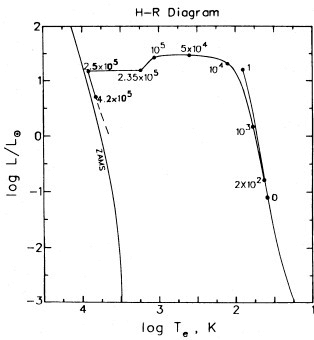
\includegraphics[width=(0.8\textwidth),height=\textheight,keepaspectratio]{premain}
\caption{Evoluzione verso inizio reazioni fusione.}
\end{figure}


Il risultato della differenza tra l'et\'a del sistema solare e il tempo impiegato dal collasso a raggiungere le condizioni per la fusione dell'idrogeno \'e il periodo trascorso dal sole in sequenza principale:

L'et\'a del sole \'e $\tsun=(4.566\pm0.005)*\sci{9}\,yr$.



\subsection{Distanza, Massa, Raggio e Luminosit\'a.}

\subsubsection{Distanza}


Il prodotto $G\msun$ \'e determinato da moti planetari quindi $\msun1.989*\sci{33}\,gr$.
\index{Distanza (fare) moderni?}

\subsubsection{Raggio}

La determinazione del raggio solare si riduce alla misura del  diametro apparente e ad un modello della regione di transizione: nota la distanza terra-sole ho una misura di $\rsun$,  un valore  rappresentativo \'e $\rsun=6.9599\sci{10}\,cm=695.99\,Mm$. Per correzioni vedi parte di inversione.

\subsubsection{Luminosit\'a}
La luminosit\'a solare misurata tramite satelliti risultante dalla media in un ciclo solare $\lsun=3.846*\sci{33}\,erg\,s^{-1}$.


\subsection{Composizione}

Caratterizzo la composizione stellare attraverso X, Y, Z che rappresentano rispettivamente abbondanza in massa di idrogeno ,elio ed elementi pesanti. Le misure spettroscopiche danno risultati accurati per elementi pi\'u pesanti dell'elio. Le linee di assorbimento dell'elio sono presenti solo negli strati superiori dell'atmosfera solare a causa delle alte energie di eccitazione. Misuro invece il rapporto $\frac{Z_s}{X_s}$ che caratterizza la composizione attuale della superficie: ho che $\frac{Z_s}{X_s}=0.0245-0.23$.




\chapter{Sistemi planetari extrasolari.}
Sistemi planetari extrasolari: introduzione.
 Sistemi extrasolari: tecniche di scoperta. 
Le caratteristiche generali dei sistemi extrasolari conosciuti. Problemi aperti. Il problema dell'abitabilita' e della ricerca della vita nell'Universo (cenni). Introduzione all'astrofisica extragalattica.L'universo: la legge di Hubble e il Big Bang (introduzione). 
Il "modello standard" di universo, e sua crisi. Teorie inflazionarie (cenni).
Distribuzione di massa su grande scala. Funzioni di correlazione. tecniche di analisi statistica: la percolazione.
\PartialToc

Distinzione pianeta/brown dwarf: $M_P\leq20M_J$, i pianeti veri e propri hanno masse $M_P\leq13M_J$.

Domande fondamentali:
\begin{itemize}
    \item Quanto \'e frequente la formazione di sistemi planetari all'atto di formazione stellare?
    \item Quanto \'e frequente la formazione di pianeti terrestri?
    \item Quanto \'e frequente la nascita della vita?
\end{itemize}

\begin{figure}[!ht]
\centering
\includegraphics[width=(0.7\textwidth),height=\textheight,keepaspectratio]{exostats}
\caption{Exoplanet detection statistic (2010).}
\end{figure}

\clearpage

\section{Moto dei pianeti.}


\begin{figure}[!ht]
\centering
\includegraphics[width=(0.7\textwidth),height=\textheight,keepaspectratio]{orbits}
\caption{orbits.}
\end{figure}

\subsection{Moto attorno al centro di massa}

Il moto di un singolo pianeta attorno ad una stella provoca un moto riflesso della stella attorno al centro di massa. Questo provoca perturbazione delle caratteristiche osservabili
\begin{itemize}
    \item Radial velocity
    \item angular (astrometric) position in the sky
    \item arrival time of periodic reference signal 
\end{itemize}

Il pianeta e la stella orbitano attorno al comune CM in orbite ellittiche chiuse con il CM come uno dei 2 fuochi.

\begin{align*}
&r=\frac{a(1-e^2)}{1+e\cos{\nu}}\\
&\frac{x^2}{a^2}+\frac{y^2}{b^2}=1\\
&b^2=a^2(1-e^2)
\end{align*}

\subsection{Anomali vera, eccentrica e media.}

Anomalia vera, $\nu(t), f(t)$: \'e l'angolo tra la direzione del pericentro e la posizione al tempo t misurata dal baricentro. L'anomalia eccentrica \'e l'angolo corrispondente all'anomalia vera riferito al cerchio ausiliario
\begin{align*}
&\cos{\nu(t)}=\frac{\cos{E(t)}-e}{1-e\cos{E(t)}}\\
&\tan{\frac{\nu(t)}{2}}=\sqrt{\frac{1+e}{1-e}}\tan{\frac{E(t)}{2}}
\end{align*}

L'anomalia medi \'e un'angolo relativo al moto medio attorno all'orbita: in un'orbita completa il pianeta non ha velocit\'a angolare costante ma una velocit\'a angolare media \'e specificata in termini del moto medio $n=\frac{2\pi}{P}$. L'anomalia media al tempo $t-t_p$ dopo il passaggio al pericentro \'e
\begin{align*}
&M(t)=\frac{2\pi}{P}(t-t_p)=n(t-t_p)\\
&M(t)=E(t)-e\sin{E(t)}
\end{align*}

\subsection{Specificazione dell'orbita.}

\begin{figure}[!ht]
\centering
\includegraphics[width=(0.7\textwidth),height=\textheight,keepaspectratio]{orbits3D}
\caption{Keplerian orbit description in 3D.}
\end{figure}

\clearpage

\subsection{Leggi di Keplero}

\begin{figure}[!ht]
\centering
\includegraphics[width=(0.7\textwidth),height=\textheight,keepaspectratio]{orbitsCM}
\caption{Two orbiting bodies.}
\end{figure}

Leggi di keplero (Original)

\begin{enumerate*}
    \item L'orbita di un pianeta \'e un'ellisse con il Sole come fuoco. (Inverse square law of gravity)
    \item Il raggio che congiunge Sole-pianeta spazza aree uguali in intervalli uguali. (Conservazione momento angolare)
    \item Il quadrato del periodo orbitale dei pianeti \'e proporzionale al cubo del semiasse maggiore. (Inverse square law of gravity)
\end{enumerate*}

Quando la massa del pianeta non \'e trascurata
\begin{equation*}
    P^2=\frac{4\pi^2}{GM}a^3
\end{equation*}

Specifico:
\begin{itemize}
    \item Orbite relative: moto del pianeta relativo alla stella.
    \begin{equation*}
    P^2=\frac{4\pi^2}{G(M_*+M_p)}a^3_{Rel}
    \end{equation*}
    dove usiamo il semiasse maggiore dell'orbita relativa.
    
    Per $M_P\ll M_*$ in unit\'a dell'orbita terrestre
    \begin{equation*}
    P\approx\SI{1}{\year}(\frac{a_{Rel}}{\si{\astronomicalunit}})\expy{\frac{3}{2}}(\frac{M_*}{\msun{}})\expy{-\frac{1}{2}}
    \end{equation*}
    
    \item Orbite assolute: per l'orbita della stella attorno al baricentro del sistema vale
    \begin{equation*}
    P^2=\frac{4\pi^2}{GM'}a_*^3
    \end{equation*}
    dove $M'=\frac{M_P^3}{(M_*+M_P)^2}$ e $a_*$ \'e il semi-asse maggiore dell'orbita stellare attorno al baricentro.
    
    Espressione equivalente per l'orbita del pianeta attorno al baricentro.
    
    Le dimensioni delle orbite sono in proporzione:
    \begin{equation*}
        a_*:a_p:a_{rel}=M_p:M_*:(M_p+M_*)
    \end{equation*}
    con $a_{rel}=a_p+a_*$, $P_{rel}=P_p=P_*$ e $e_{rel}=e_p=e_*$.
    
\end{itemize}



\clearpage

\section{Metodi per la scoperta di sistemi planetari extrasolari.}

\subsection{Metodi diretti.}

Risoluzione del sistema in maniera visuale: la separazione angolare Sole/Giove sarebbe \SI{1}{\arcsec} gi\'a a \SI{5}{\parsec}.

Estrema differenza tra $L^*$ e $L_P$: per il sistema Sole/Giove nel visibile
\begin{align*}
    \frac{L_P}{L_*}=P(\lambda,\alpha)(\frac{R_P}{a})^2\approx\num{e-9}&\intertext{$P(\lambda,\alpha)$ dipende da albedo e fase a cui si trova il pianeta.}
\end{align*}

Effetto di selezione: pianeti lontani dalla stella ($a>\SI{10}{\astronomicalunit}$).

\subsection{Timing}

Se luce emessa dalla stella primari ha tempi caratteristici il moto ellittico dovuto alla presenza del pianeta produce variazioni nel cammino ottico della luce proporzionaleallo spostamento della primaria lungo la linea di vista
\begin{equation*}
    \tau_p=\frac{1}{c}\frac{a\sin{i}M_p}{M_*}
\end{equation*}

\subsubsection{Osservazioni di pulsar.}

Emettono segnale periodico regolare $\Pi\approx\si{\second}-\si{\milli\second}$. Il moto attorno al comune centro di massa Pulsar/pianeta causa una variazione del cammino ottico: il segnale arriva in anticipo o in ritardo.

Nel caso de lsistema Sole/Terra il sole percorre un'ellisse di semiasse maggiore circa \mblock{\frac{m_T}{\msun{}}a_T\approx\SI{500}{\kilo\meter}}: la differenza di cammino ottico causerebbe un $\Delta t\approx\SI{1}{\milli\second}$.

Sistemi non nati con la stella: formati in fase finale di evoluzione.

\subsection{Microlensing gravitazionale.}

La presenza di materia (densit\'a di energia) distorce lo spazio-tempo e il la radiazione EM pu\'o essere deviata: la luce proveniente da un'oggetto lontano pu\'o essere deviata dal campo gravitazionale di un oggetto (lente) e quindi per l'oservatore risulta distorta e amplificata. 

\begin{definition}{Microlensing.}
Si parla di microlensing quando le immagini multiple dell'oggetto lontano non sono risolte.
\end{definition}

\subsubsection{Gravitational light bending}

\begin{definition}{Raggio di \sch{.}}
Il raggio di \sch{} \'e
\begin{equation*}
    R_S=\frac{2GM_L}{c^2}
\end{equation*}
\end{definition}

\begin{figure}[!ht]
\centering
\includegraphics[width=(0.9\textwidth),height=\textheight,keepaspectratio]{lensing}
\caption{lensing.}
\end{figure}

\begin{align*}
&\alpha_{GR}=\frac{4GM_L}{c^2b}=\frac{2R_S}{b}&\intertext{con la condizione che il parametro di impatto $b\gg R_S$}
\end{align*}

Lens equation
\begin{equation*}
\theta_S=\theta_I-2R_S\frac{D_{LS}}{D_LD_S}\frac{1}{\theta_I}
\end{equation*}

\clearpage

\subsubsection{Einstein radius.}

La sorgente lontana vedra la sua luminosit\'a amplificata dalla lente in proporzione all'Anello di Einstein
\begin{equation*}
    \theta_E^2=\frac{4GM_LD_{LS}}{c^2D_{OL}D_{OS}}
\end{equation*}

\begin{figure}[!ht]
\centering
\includegraphics[width=(0.7\textwidth),height=\textheight,keepaspectratio]{microlensing}
\caption{Curva di luce per microlensing.}
\end{figure}

Le sorgenti galattiche possono essere stelle del nucleo galattico ($D_{OS}\approx\SI{10}{\kilo\parsec}$ e lenti tipic a met\'a strada).

Per $M_L\approx\msun{}$: $\theta_E\approx\si{\milli\arcsec}$.

Le dimensioni dell'anello di Einstein definiscono il livello di allineamento richiesto per avere una significativa amplificazione del segnale della sorgente.

Dimensioni lineari dell'anello di Einstein
\begin{align*}
    R_E=(1-y)\,d\theta=\sqrt{2y(1-y)R_Sd}
\end{align*}
con $d=D_{os}$, $yd=D_{LS}$, massime dimensioni lineari per $y=\frac{1}{2}$.
Il raggio di luce deve passare ad una distanza inferiore di $R_E$ dalla lente.

Inserendo quantit\'a tipiche per ricerca di esopianeti
\begin{align*}
&\theta_E\approx1.0(\frac{M_L}{\msun{}})\expy{\frac{1}{2}}(\frac{D_L}{\SI{8}{\kilo\parsec}})\expy{-\frac{1}{2}}(\frac{D_{LS}}{D_S})\expy{\frac{1}{2}}\si{\milli\arcsec}\\
&R_E\approx8.1(\frac{M_L}{\msun{}})\expy{\frac{1}{2}}(\frac{D_S}{\SI{8}{\kilo\parsec}})\expy{\frac{1}{2}}(\frac{D_LD_{LS}}{D_S^2})\expy{\frac{1}{2}}\si{\astronomicalunit}
\end{align*}

\subsubsection{Magnification}

\begin{figure}[!ht]
\centering
\includegraphics[width=(0.7\textwidth),height=\textheight,keepaspectratio]{lensinglcurves}
\caption{Microlensing magnification.}
\end{figure}

\clearpage

Fatti:
\begin{itemize}
    \item In un cilindro di raggio $R_E$ e altezza $D_{OS}$ ho probabilit\'a $\frac{1}{100000}$ che ci sia una stella.
    \item Se la lente \'e costituita da pi\'u masse avremo una curva di luce con pi\'u picchi
    \item Nel caso di lente con sistema planetario la distribuzione dei picchi \'e detrminata dalla posizione dei pianeti: pi\'u efficace vicino all'anello di Einstein.
\end{itemize}

\begin{figure}[!ht]
\centering
\includegraphics[width=(0.7\textwidth),height=\textheight,keepaspectratio]{mp-a-micro}
\caption{Massa pianeti vs semiasse per pianeti scoperti tramite microlensing.}
\end{figure}

\clearpage

\subsection{Tecniche astrometriche}

Misura posizione e moti dei corpi celesti. The path of a star orbiting star-planet barycentre appears projected on the plane of the sky as an ellipse with angular semi-major axis $\alpha$
\begin{align*}
&a_*:a_{rel}=M_p:(M_p+M_*),\ a_{rel}=a_*+a_p
&\alpha=\frac{M_p}{M_*+M_p}a\approx\frac{M_p}{M_*}a\\
&\approx(\frac{M_p}{M_*})(\frac{a}{\SI{1}{\astronomicalunit}})(\frac{d}{\SI{1}{\parsec}})\expy{-1}\si{\arcsec}
\end{align*}


\subsection{Tecniche spettroscopiche (Misura velocit\'a radiale).}

Variazione periodica della velocit\'a radiale dovuta al moto attorno al CM.

For the radial velocity semi-amplitude we have
\begin{align*}
&v_r=K[\cos{\omega+\nu}+e\cos{\omega}]\\
&K=\frac{2\pi}{T}\frac{A_*\sin{i}}{\sqrt{1-e^2}}\\
&K^2=\frac{G}{(1-e^2)}\frac{1}{a_*\sin{i}}\frac{M_p^3\sin^3{i}}{(M_*+M_p)^2}&\intertext{radial velocity measurement provide a value for mass function}\\
&\frac{M_p^3\sin^3{i}}{(M_*+M_p)^2}
\end{align*}

La terza legge di Keplero
\begin{equation}
(M^*+m_P)\sin^3{i}=\frac{4\pi^2a^3\sin^3{i}}{GP^2}
\end{equation}

$i$ \'e l'inclinazione dell'orbita rispetto al piano nella sfera celeste normale alla linea di vista.

Se entrambi gli spettri fossero osservabili dalle velocit\'a radiali ottengo $a^*\sin{i}, a_P\sin{i}$ e $(M^*+m_P)\sin^3{i}$ essendo $\frac{a^*\sin{i}}{a_P\sin{i}}=\frac{m_P}{m^*}$: ottengo $M^*\sin{i}$ e $m_P\sin{i}$.

Nel caso usuale in cui sia osservabile solo lo spettro della stella:

\begin{align*}
&a=a^*+a_P=a^*(1+\frac{a_P}{a^*})=a^*(1+\frac{M^*}{m_P})\\
&a^3\sin^3{i}=a^*\sin^3{i}(\frac{m_P+M^*}{m_P})^3
\end{align*}

Definisco la funzione delle masse
\begin{align*}
&f(M^*,m_P)=(M^*+m_P)\sin^3{i}\frac{m_P^3}{(M^*+m_P)^3}\\
&=\frac{4\pi^2}{GP^2}{a^*}^3\sin^3{i}\\
&f=\frac{PK_2^3}{2\pi G}&\intertext{$K_2$ is half the change in radial velocity.}\\
&f=\frac{M_1\sin^3{i}}{(1+q)^2}&\intertext{q \'e il rapporto tra le masse $M^*$ fratto massa oggetto non visibile $m_P$.}
\end{align*}

Se il sistema \'e anche fotometrico \'e possibile valutare l'inclinazione; ponendo $i=\frac{\pi}{2}$ ho un limite inferiore per le masse.

Ampiezza variazione velocit\'a radiale massa stella host
\begin{equation*}
v=\frac{30m_P\sin{i}}{{M^*}\expy{\frac{2}{3}}P\expy{\frac{1}{3}}},\ \si{\kilo\meter\per\second}
\end{equation*}
dove la massa \'e espressa in $\msun{}$ e il periodo in anni: posso ricavare $m_P\sin{i}$.

Per il sistema Sole/Giove $v\approx\SI{12}{\meter\per\second}$.

Sole/Terra $v\approx\SI{10}{\cm\per\second}$.

Prendendo la coordinata z della stella lungo la linea di vista
\begin{align*}
&z=r(t)\sin{i}\sin{(\omega+\nu)}\\
&v_r=\dot{z}=K[\cos{(\omega+\nu)}+e\cos{\omega}]\\
&K=\frac{2\pi}{P}\frac{a_*\sin{i}}{(1-e^2)\expy{\frac{1}{2}}}
\end{align*}

\begin{figure}[!ht]
\centering
\includegraphics[width=(0.9\textwidth),height=\textheight,keepaspectratio]{vrcurve}
\caption{Stellar radial velocity curves: dependency on $e$ and $\omega$.}
\end{figure}

\clearpage

\subsection{Tecniche fotometriche: transiti.}

\begin{figure}[!ht]
\centering
\includegraphics[width=(0.9\textwidth),height=\textheight,keepaspectratio]{transit}
\caption{Schematic of a transit and secondary eclipse (planet passes behind).}
\end{figure}

Abbiamo 4 osservabili
\begin{itemize}
    \item Il periodo P.
    \item La profondit\'a del transito $\Delta F$.
    \item Intervallo di tempo tra 1-4 $t_T$.
    \item Intervallo di tempo tra 2-3 $t_F$.
\end{itemize}


\begin{align*}
&\Delta F\approx(\frac{R_p}{R_*})^2\\
&t_T\approx13(\frac{M_*}{\msun{}})\expy{-\frac{1}{2}}(\frac{a}{\si{\astronomicalunit}})\expy{\frac{1}{2}}\frac{R_*}{\rsun{}}\si{\hour}
\end{align*}

La probabilit\'a che per un pianeta orientato arbitrariamente si possa osservare transito a eclisse secondaria \'e
\begin{equation*}
Pr\frac{R_*}{a}\approx0.005\frac{R_*}{\rsun{}}(\frac{a}{\si{\astronomicalunit}})\expy{-1}
\end{equation*}
data dall'area spazzata dall'ombra del pianeta sulla sfera celeste.

\begin{figure}[!ht]
\centering
\includegraphics[width=(0.7\textwidth),height=\textheight,keepaspectratio]{transitex}
\caption{Transito visto dalla Terra.}
\end{figure}

\begin{figure}[!ht]
\centering
\includegraphics[width=(0.7\textwidth),height=\textheight,keepaspectratio]{sphereshadow}
\caption{Area della sfera celeste su cui \'e proiettato il transito.}
\end{figure}

Fatti:
\begin{itemize}
    \item Per un'eclissi totale Sole/Giove ho variazione $\Delta L\approx1\%$.
\end{itemize}

\begin{figure}[!ht]
\centering
\includegraphics[width=(0.7\textwidth),height=\textheight,keepaspectratio]{mp-atransit}
\caption{Massa pianeta vs semiasse per pianeti scoperti tramite transito.}
\end{figure}

\clearpage

\section{Caratteristiche e problemi interpretativi.}

\begin{figure}[!ht]
\centering
\includegraphics[width=(0.7\textwidth),height=\textheight,keepaspectratio]{mp-a}
\caption{Massa pianeti vs semiasse .}
\end{figure}

\subsection{Caratteristiche preferenziali della stella primaria??}

\begin{equation*}
\frac{\parbox{0.8\textwidth}{$\#$ Sistemi osservati che hanno pianeti}}{\parbox{0.8\textwidth}{$\#$ Sistemi osservati}}
\end{equation*}

''A livello preliminare si oserva una carenza di pianetti attorno a stelle doppie.''

Ci sono caratteristiche delle stelle che rendono pi\'u probabile la formazione di pianeti?

\begin{figure}[!ht]
\centering
\includegraphics[width=(0.8\textwidth),height=\textheight,keepaspectratio]{mp-a-micro}
\caption{Massa stella primaria.}
\end{figure}

\begin{figure}[!ht]
\centering
\includegraphics[width=(0.8\textwidth),height=\textheight,keepaspectratio]{mp-a-micro}
\caption{Metallicit\'a stella primaria.}
\end{figure}

\clearpage

\subsection{Modello formazioni pianeti di Sovronof.}

Formazione pianeti a partire da grani solidi della nube proto-planetaria: privilegia sistemi ad alta metallicit\'a, daltra parte l'alta metallicit\'a della stella potrebbe essere causata dalla caduta di materia (pianeti) su di essa.

Pianeti attorno a stelle con bassa metallicit\'a indicherebbe la presenza di pi\'u canali di formazione.

Effetti di selezione: stelle con $M^*<\msun{}$ sono studiate di meno.


\subsection{Distribuzione di massa dei pianeti.}

La distribuzione di massa dei pianeti \'e piccata attorno a $M_J$ e il $60\%$ dei pianeti hanno massa $m_P<2M_J$.

L'assenza di pianeti con $m_P\gg M_J$ \'e indizio di separazione tra processi di formazione planetaria e quelli stellari che non coinvolgono in maniera dominante la componente polverosa.

L'efficienza dei processi di migrazione rendono difficile la sopravvivenza di Brown dwarf vicino alla primaria.


\subsection{Distribuzione semi-assi maggiori.}

La maggior parte dei pianeti scoperti\'e pi\'u interna di Giove : in molti hanno a inferiore a quello terrestre.

Hot Jupiters: pianeti estremamente vicini alla stella.

Effetti di selezione:
\begin{itemize}
    \item Sistemi larghi: imaging.
    \item Sistemi stretti: transiti.
\end{itemize}

\begin{figure}[!ht]
\centering
\includegraphics[width=(0.8\textwidth),height=\textheight,keepaspectratio]{e-a}
\caption{Eccentricit\'a vs semiasse.}
\end{figure}

\begin{figure}[!ht]
\centering
\includegraphics[width=(0.8\textwidth),height=\textheight,keepaspectratio]{e-adistant}
\caption{Eccentricit\'a vs semiasse sistemi distanti.}
\end{figure}

\clearpage

\subsection{Confronto con modelli di formazione sistema solare.}

Modello dominante: aggregazione di pianeti partendo nuclei solidi di polvere o ghiaccio presenti nella nebulosa proto solare.

Pianeti giaganti in posizioni non arbitrarie: oltre l'orbita di Marte.

Processi migrazione planetaria:
\begin{itemize}
    \item Interazione disco proto-planetario/pianeta
    \item Jumping jupiters (:orbite eccentriche??)
    \item A distanza troppo piccola l'interazione mareale stella-pianeta induce forte circolarizzazione delle orbite.
\end{itemize}


\chapter{Galassie. Universo extra-galattico.}
Le galassie; metodi di stima delle distanze; il diagramma di Hubble e considerazioni generali.

L'universo extragalattico: distribuzione della brillanza. Nuclei attivi, quasars. Introduzione alla radioastronomia.
L'universo extragalattico (conclusione). 
\PartialToc

%https://en.wikipedia.org/wiki/Galaxy_morphological_classification

\section{Problematiche: nubi interstellari, galassie.}


Hubble scopri\'e variabili di tipo Cefeidi in Andromeda ed in altre galassie a spirale: parte degli oggetti estesi osservabile erano galassie a grande distanza.

Oggetti estesi osservabili:
\begin{itemize}
\item Nubi interstellari galattiche:
    
hanno estensione di qualche \si{\parsec} e distanza qualche \si{\kilo\parsec}.
\item Galassie:
    
hanno estensione di qualche \si{\kilo\parsec} e distanze maggiori del \si{\mega\parsec} (dimensioni angolari: minuti-gradi).
\end{itemize}

Hubble stima la distanza applicando la relazione $\Pi-L$ delle Cefeidi e altre stelle pulsanti con $\Pi\approx1^d$.

\subsection{Osservabilit\'a di una stella pulsante in una galassia esterna.}

Limiti da Terra:
\begin{itemize}
\item Potere risolutivo ottico del telescopio $\frac{\lambda}{D}$.
\item Seeing atmosferico: risoluzione massima \SI{1}{\arcsec}.
\end{itemize}

Fondo stellare galattico.

Le dimensioni trasversali di un parallelepipedo di base quadrata con dimensioni sulla sfera celeste di $\SI{1}{\arcsec}\times\SI{1}{\arcsec}$ aumentano in maniera proporzionale a $r^2$.

La luminosit\'a assoluta risulta dalla somma su tutte le sorgenti luminose presenti in quel volume e quindi a parit\'a di tipologia di oggetto osservato aumenta come $r^2$: bilancia la diminuzione di luminosit\'a osservata come $\frac{1}{r^2}$.

\begin{definition}{Brillanza di una galassia.}
Magnitudine apparente della minima superficie risolta.
\end{definition}

Fatti:

La brillanza di una galassia \'e indipendente dalla distanza.

\subsubsection{Toy model di galassia.}

Direzione di osservazione parallela all'asse polare della galassia e distanza dalla galassia \SI{1}{\mega\parsec}.

\num{e10} Soli distribuiti su un disco di \SI{10}{\kilo\parsec} di raggio.

In un quadrato $\ang{;;1}\times\ang{;;1}$ osserviamo le stelle nel parallelepipedo di altezza pari allo spessore del disco e come alto di base \mblock{\SI{1}{\mega\parsec}*(\frac{\ang{;;1}}{\SI{1}{\radian}})=\SI{5}{\parsec}} che comprende una frazione \mblock{\frac{25}{\pi\num{e8}}\approx\num{e-7}} delle stelle totali cio\'e circa \num{e3} stelle. A distanza di \SI{1}{\mega\parsec}
\begin{equation*}
    m_{V\odot}=M_{V\odot}+5\log{\frac{\SI{1}{\mega\parsec}}{\SI{10}{\parsec}}}\approx29.7
\end{equation*}

la magnitudine apparente di \num{e3} stelle sarebbe 

\begin{equation*}
m_V=29.7-2.5\log{1000}=22
\end{equation*}

valore realistico per zone non troppo centrali o periferiche.

Una stelle di magnitudine 22 pu\'o corrispondere a una stella di $M_V=-3$ a \SI{1}{\mega\parsec} o $M_V=-8$ a \SI{10}{\mega\parsec}.

Fatti:
\begin{itemize}
    \item L'osservazione di Cefeidi da Terra \'e possibile fino a distanze dell'ordine di \si{\mega\parsec}.
    \item Un fattore 10 in risoluzione fa guadagnare un fattore 100 in luminosit\'a equivalente a 5 magnitudini.
    \item La luce proveniente da una stella simile al Sole a \SI{1}{\mega\parsec} \'e molto minore di un fotone al secondo.
\end{itemize}


\subsection{Misura distanza tramite candela campione.}

\begin{itemize}
    \item Uso di supernovae di tipo I come candela campione. Assunzione: In ogni galassia la stella variabile pi\'u luminosa ha la stessa luminosit\'a assoluta.
    
    Evento raro.
    
    Misura desine di \si{\mega\parsec}.
    \item Le galassie hanno tutte la stessa luminosit\'a.
    \item Le galassie pi\'u luminose di ciascun cluster hanno la stessa luminasit\'a: nelle zone centrali degli ammassi pi\'u grandi fenomeni di merging danno vita ad oggetti massicci e luminosi in maniera anomala.
\end{itemize}

\section{Propriet\'a complessive delle galassie.}
Vedi: The mass distribution in the galactic disc – I. A technique to determine the integral surface mass density of the disc near the Sun.
\subsection{Dispersione della velocit\'a delle stelle.}

La velocit\'a delle stelle \'e legata tramite il viriale al potenziale gravitazionale e quindi alla massa totale

\subsection{Relazioni di Tully-Fisher.}

Relazioni $V/L$.

\subsection{Correzione di Baade per la distanza delle galassie vicine.}

Le dimensioni delle galassie vicine sono paragonabili alla nostra.

Sono presenti tipi diversi di Cefeidi con differenti relazioni $\Pi/L$.

\section{Classificazione delle galassie. Luminosit\'a e spettroscopia.}

\subsection{Diagramma di Hubble.}

\begin{figure}[!ht]
\centering
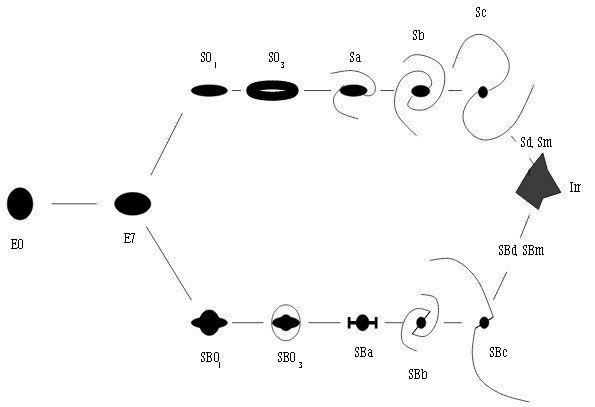
\includegraphics[width=(0.8\textwidth),height=\textheight,keepaspectratio]{galaxiesH}
\caption{Diagramma di Hubble.}
\end{figure}

Fatti:
\begin{itemize}
    \item Ellittiche: E.
    
    Le ellittiche son caratterizzate dal numero \mblock{n=10(1-\frac{b}{c})}, dove b e csono gli assi apparenti dell'ellissi proiezione.
    
    \item Le S0 si distinguono dalle ellittiche per una pi\'u lenta decrescita della luminosit\'a al di fuori della zona centrale: struttura esterna appiattita.
    
    \item Le spirali S sono caratterizzate da una struttura a disco articolata in bracci di maggiore addensamento stellare. Le lettere a,b,c indicano una minor importanza del nucleo centrale e crescente apertura delle braccia (nelle quali si individuano meglio $HII$ regions).
\end{itemize}

\clearpage

\subsection{Classificazione di Yerkers.}

\begin{itemize}
\item B	Barred spirals.
\item D	Galaxies with rotational symmetry but showing neither spiral structure nor ellipticity.
\item cD	Supergiant D galaxies, predominantly found in clusters and embedded in an extensive halo.
\item db	Dumb-bell systems.
\item E	Ellipticals.
\item Ep	Peculiar ellipticals containing conspicuous absorbtion patches.
\item I	Irregulars.
\item L	Low-surface-brightness systems.
\item N	High-luminosity nucleus superimposed on a considerably fainter outer envelope.
\item Q	Quasi-stellar objects.
\item S	Ordinary spirals.
\end{itemize}


\subsection{Spettroscopia delle galassie.}

Il tipo spettrale di una galassia \'e determinato dal tipo spettrale medio delle stelle cha ne fanno parte e dai contributi della materia diffusa e dall'arrossamento interstellare.

Nel diagramma di Hubble abbiamo le ellittiche con stelle di tipo K: $(B-V)\approx1$, spirali con stelle di tipo F e irregolari con stelle di tipo A.

Nelle galassie irregolari sono presenti abbondanti processi di formazione stellare recenti, scarsi nelle ellittiche.

Le righe spettrali sono disperse a causa dell'effetto Doppler: il moto orbitale (solo in parte Kepleriano) \'e caratterizzato da $v\approx\SI{100}{\kilo\meter\per\second}$ (l'effetto pu\'o essere ridotto se l'osservazione \'e localizzatain una regione con velocit\'a relative piccole).

\subsection{Distribuzione spaziale della luminosit\'a.}

Considero la galassia come un gas di stelle.

\begin{definition}{Brillanza superficiale (galassia).}
Luminosit\'a per angolo solido: $\mu=\si{\magnitude\per\squared\arcsec}$.
\end{definition}

La brillanza non dipende dalla distanza.

\begin{itemize}
    \item Galassie giganti: $\mu_B\approx17$.
    \item Galassie medie: $\mu_B\approx22$.
    \item Fondo cielo: $\mu>26$.
\end{itemize}

\begin{definition}{Magnitudine totale (galassia).}
La magnitudine totale della galassia \'e data dall'integrazione del profilo di brillanza fino all'isofota del fondo.
\end{definition}

Magnitudini assolute:
\begin{itemize}
    \item Galassie giganti: $M_V\approx\numrange{-20}{-25}$.
    \item Galassie nane: $M_V\approx\numrange{-15}{-10}$.
\end{itemize}
Si ottengono determinando la distanza tramite candele standard o legge di Hubble (Red Shift).

Determinazione raggio.

Isofota critica definisce il raggio di Holmberg a $\SI{26.5}{\magnitude\per\square\arcsec}$.


\subsection{Profilo di brillanza delle galassie ellittiche.}

\subsubsection{Galassie ellittiche nane.}

Il profilo delle galassie ellittiche nane \'e simile a quello degli ammassi globulari: curve di King.

Le curve di King  sono ottenute mediante modello teorico per il gas di stelle e quindi la distribuzione risultante da una proiezione sulla sfera celeste.

Le curve di King costituiscono una famiglia a 3 parametri:

\begin{align*}
&\Sigma_0,\ r_c&\intertext{ sono la brillanza centrale e il raggio del nucleo definito da $\Sigma(r_c)=\frac{\Sigma_0}{2}$, entrambi osservati e definito il raggio per cui $\Sigma(r_T)=0$}\\
c=\log{\frac{r_T}{r_c}}&\intertext{ricavato tramite best fit.}
\end{align*}

Per c piccolo la distribuzione di massa \'e rapidamente troncata, per c infinitamente grande si ha una distribuzione di massa che va a zero asintoticamente (sfera isoterma).

\subsubsection{Galassie ellittiche giganti.}

La situazione \'e pi\'u complessa. Formula empirica di de Vaucoulurs
\begin{equation*}
\Sigma(r)=\Sigma_e10\expy{-3.33[(\frac{r}{r_e})\expy{\frac{1}{4}}-1]}
\end{equation*}
$r_e$ \'e il raggio efficace determinato attraverso la mediana della distribuzione di brillanza
\begin{equation*}
2\int_0^{r_e}\Sigma(r)2\pi r\,dr=7.22\pi r_e^2\Sigma_e
\end{equation*}
con $\Sigma_e=\Sigma(r_e)$.

Generalizzazione: $\frac{1}{4}\to\frac{1}{n}$ diverso da galassia a galassia.

\subsection{Profilo di brillanza delle galassie a spirale.}

Somma di due componenti:
\begin{itemize}
    \item Bulge (nucleo): andamento alla de Vaucouleurs
    \item Contributo del disco: $\Sigma(r)=\Sigma(r_s)\exp{-\frac{r}{r_s}}$.
\end{itemize}

Il rapporto tra emissione del disco e del bulge \'e $\frac{D}{B}=0.28(\frac{r_s}{r_e})^2\frac{\Sigma(r_s)}{\Sigma_e}$.

\section{Radio-Galassie e quasar.}

\subsection{Galassie di Seyfert.}

Forti righe di emissione.

\subsection{Galssie N.}

Nucelo molto pi\'u brilante del resto.

\subsection{BL Lacertae.}

Visibili solo i nuclei.

\subsection{QSO: quasi-stellar object. Quasar}

Emissione radio \'e legata ad intensi campi EM e a processi tipo radiazione di sincrotrone. Emissione non termica.

La brillanza radio non \'e correlata a quella ottica.

Zone emissione radio: strutture anche estese circostanti il nucleo galattico.

\subsubsection{Quasar}

Le quasar sono oggetti estremamente luminosi e distanti.

Fotometria: eccesso ultravioletto ed infrarosso (non presente in nane bianche o in variabili irregolari).

Spettroscopia: alto red-shift legato all'espansione dell'universo.

\section{Struttura dell'universo su grande scala.}

Cosmolgia: galassie sono le particelle fondamentali, studia la geometria spazio-temporale e la distribuzione di materia nello spazio.

\subsection{Legge di Hubble.}

Chiamo $\vec{r}$ la posizione dell'osservatore, $\vec{v}$ la velocit\'a relativa all'osservatore della sorgente, il vettore $\vec{\phi}$ termine di velocit\'a peculiare della sorgente sofrapposto al flusso di Hubble:
\begin{equation*}
    \vec{v}=H\vec{r}+\vec{\phi}
\end{equation*}
$H$ \'e la costante di Hubble dimensioni di \si{\per\second}: $H\approx\frac{1}{\tau_U}\SI{e-10}{\year}$, usualmente misurata in \si{\kilo\meter\per\second\per\mega\parsec}, $H=\SIrange{60}{70}{\kilo\meter\per\second\per\mega\parsec}$.

Il temine peculiare \'e di entita\'a limitata: per oggetti di stanti pi\'u di \SI{10}{\mega\parsec} il termine di espansione domina sul peculiare $\vec{v}\propto\vec{r}$.

\subsection{Organizzazione gerarchica delle disomogeneit\'a.}

L'universo diventa pi\'u omogeneo all'aumentare della scale: il contrasto di densit\'a tra varie regioni tende a diminuire. Un modello globale ragionevole \'e omogeneo e isotropo.

Organizzazione gerarchica delle disomogeneit\'a:
\begin{enumerate}
\item Galassie.
\item Cluster: ammssi di dimensione intorno al \si{\mega\parsec}.
\item Super-ammassi: scala di \SI{10}{\mega\parsec}.

Filamenti o superfici di densit\'a superiore alla media.
\end{enumerate}

Studio evoluzione sulla base della struttura passata desumibile dalla radiazione di fondo (quando era 1000 volte pi\'u piccolo).

Studio clusterizzazione 3D, esistenza di superfici ad alta densit\'a di galassie e filamenti 1D.

\subsubsection{Termine di correlazione.}

In un volume di universo V ci sono N galassie.

La probabilit\'a di trovare una galassia in $dV$ \'e $P=n\,dV=\frac{N}{V}\,dV$. Per una distribuzione casuale  $P_{12}=n^2\,dV_1\,dV_2$ \'e la probabilit\'a di trovare i volumi $dV_1$ e $dV_2$ popolati.

Per distribuzione non casuale introduco termine di correlazione che per invarianza traslazionale e rotazionale dipende solo dalla distanza tra $dV_1$ e $dV_2$:

\begin{equation*}
    P_{12}=n^2[1+\epsilon(r)]\,dV_1\,dV_2
\end{equation*}

$\epsilon(r)>0$ implica l'esistenza di cluster.

\subsubsection{Toy model: universo quadrato.}

Considero un quadrato di lato L e tutta la materia \'e in quadrato $\frac{L}{4}$:

prendendo un punto a caso $x_1$ la probabilit\'a che sia popolato \'e $\frac{1}{16}$, prendendo un punto $x_2$ a piccola distanza $r\ll l$ \'e probabile che sia nello stesso cluster/regione vuota di $x_1$
\begin{equation*}
    \epsilon(r)=\left\{\begin{array}{cc}
         \frac{1}{16}(256-1)+\frac{15}{16}(-1)=15 & \text{ per } r\ll l \\
         -1 & \text{ per } r\gg l\\
    \end{array}\right.
\end{equation*}

Osservativamente:
\begin{equation*}
    \epsilon_{gal}(r)=(\frac{r}{r_0})\expy{-\gamma}
\end{equation*}
con $r_0\approx\SI{5}{\mega\parsec}$ e $\gamma\approx1.8$. La relazione osservativa conferma struttura clusterizzata con lunghezza di correlazione del'ordine del \si{\mega\parsec}.

Per gli ammassi:
\begin{equation*}
    \epsilon_{cl}(r)=(\frac{r}{r_1})\expy{-\gamma}
\end{equation*}
con $r_1\approx\SI{25}{\mega\parsec}$.

\subsubsection{Test di percolazione.}

Il test di percolazione \'e utile per cercare strutture 1D.

\begin{figure}[!ht]
\centering
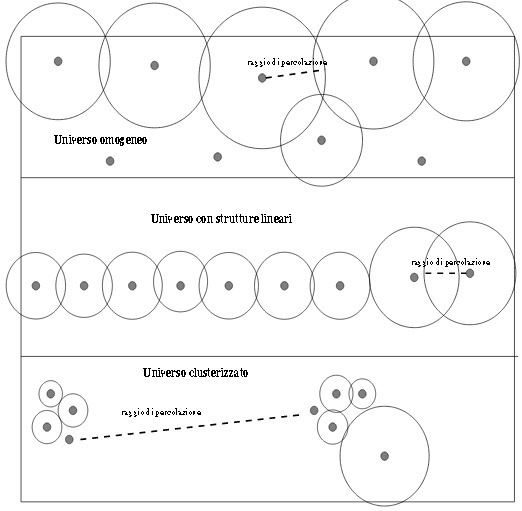
\includegraphics[width=(0.9\textwidth),height=\textheight,keepaspectratio]{percolazione}
\caption{Test di percolazione.}
\end{figure}

Definisco il raggio di percolazione come il raggio per cui preso un insieme di galassie, ognuna circondata da una sfera di tale raggio, ottengo strutture connesse che mi permettono di attraversare il volume dato di universo

\begin{equation*}
    r_{Perc}\left\{\begin{array}{cc}
                =n\expy{-\frac{1}{3}}&\text{distribuzione uniforme}\\
                >n\expy{-\frac{1}{3}}&\text{Cluster}\\
                <n\expy{-\frac{1}{3}}&\text{Struttura 1D o 2D.}\\
    \end{array}\right.
\end{equation*}

\clearpage

\renewcommand{\listfigurename}{Elenco figure}
\renewcommand{\indexname}{Indice}

\listoffigures
\printindex


\end{document}